\documentclass{article}
\usepackage{listings}
\usepackage[margin=1in]{geometry}
\usepackage{graphicx}
\usepackage[pdftex,hypertexnames=false,bookmarks=true,linkbordercolor={.9 .9 1}]{hyperref} 

\title{
  
\includegraphics[width=.43\columnwidth]{codecontracts_SM.png}
\\
Code Contracts User Manual
}
\author{Microsoft Corporation}

\newenvironment{quotedText}{\begin{quote}}{\end{quote}}
\newcommand{\code}[1]{\lstinline{#1}}
\newcommand{\csharp}{C\#}
\newcommand{\comment}[1]{}
\newcommand{\requires}[1]{\code{Requires}$\langle$#1$\rangle$}
\newcommand{\requiresn}[1]{{Requires}$\langle$#1$\rangle$}
\newcommand{\EnsuresOnThrow}[1]{{EnsuresOnThrow}$\langle$#1$\rangle$}

\begin{document}
\maketitle

\noindent 
\textbf{What's New?}
\begin{itemize}
\item We fixed the debug information generated by the rewriter for async and iterator methods so that locals now appear again when debugging.
\item Static checker has a new option to warn about missing requires on methods visible outside your assembly. See Section~\ref{sec:staticcheckingoptions}.
\item The static checker recognizes a new contract helper \code{AssumeInvariant} that allows you to assume the invariant of an object at arbitrary points in your program. It is a work-around for some static checker limitations. See Section~\ref{sec:assumeinvarianthelper}.
\end{itemize}
\textbf{What was new?}
\begin{itemize}
\item Section~\ref{sec:async} describes how postconditions are handled for
async methods and methods returning tasks in general.
\item Section~\ref{sec:Inference} describes the inference options 
\item Section~\ref{sec:relevantWarnings} describes the new slider to filter relevant warnings.
\item Section~\ref{sec:filteringstaticcheckerwarnings} has been updated to describe 
the new \code{InvariantInMethod} modifier to suppress  invariant warnings at method exits.
\item You can now enable the caching of the analysis results, to avoid the re-analysis of methods that did not changed among different builds.
See Section~\ref{sec:caching}.
\item   Section~\ref{sec:filteringstaticcheckerwarnings} has been updated to describe 
the new \code{EnsuresInMethod} modifier to suppress  precondition
warnings at all call sites.
\item Section~\ref{sec:runtimecontractbehavior} clarifies the behavior
  of \code{if-then-throw} and \requires{E} with respect to the option
  \emph{assert on failure}. 
\item Section~\ref{sec:filteringstaticcheckerwarnings} has been updated to describe 
the new \code{RequiresAtCall} modifier to suppress  precondition
warnings at all call sites.
\item For each assembly, you now need to specify an explicit assembly
  mode according to how contracts are used on that assembly. See Section~\ref{sec:usage}.
\item \code{[ContractArgumentValidator]} methods support factoring legacy
  if-then-throw style parameter validation into helper methods, while
  still permitting the tools to recognize them. See Section~\ref{sec:contractargumentvalidators}.
\item \code{[ContractAbbreviator]} methods support factoring commonly
  used combinations of \code{Requires} and \code{Ensures} into helper
  methods that can be used from multiple places. See
  Section~\ref{sec:contractabbreviators}.
\item Section~\ref{sec:contractoption} describes how to turn
  off contract checking or inheritance at assembly, type, or method
  level using attributes. 
\item Section~\ref{sec:migration} describes how to migrate an existing
  project to take advantage of contracts.
\item Section~\ref{sec:testharness} describes how to deal with test
  harness setup in VS2010 when the code under test is built with .NET
  v3.5 and the \code{Microsoft.Contracts.dll}.
\end{itemize}

\tableofcontents

\pagebreak

\newcommand\codefamily\sffamily
\lstset{language={[Sharp]C},mathescape=true,showstringspaces=false,flexiblecolumns=true,morekeywords={alloc,delay,delete,expose,let,unsatisfiable,receive,rep,contract,message,state,one},basicstyle=\codefamily\small,literate={->}{{$\rightarrow$}}{2}{<<}{{$\langle$}}{2}{>>}{{$\rangle$}}{2}{!}{{\textbf{!}}}{2},frame=lines,moredelim=[is][\itshape]{@}{@},captionpos=b,numberstyle=\tiny,stepnumber=1,numbersep=2pt}

\section{Code Contracts Library Overview}
Contracts allow you to express preconditions, postconditions and object
invariants in your code for runtime checking, static analysis, and
documentation.  This document covers how to author them in your code,
and contains guidelines for using them effectively with the provided tools.

All of the contract methods are static methods defined in the
\code{Contract} class which appears in the
\code{System.Diagnostics.Contracts} namespace. 

\begin{quotedText}
Starting with the CLR v4 (or Silverlight 4), the \code{Contract} class and related types reside in
mscorlib.dll.

If you build against a platform that does not contain the Contract namespace by
default, first try to add the reference from within VisualStudio to \code{Microsoft.Contracts}
from the add reference dialog under the .NET tab. If you can't find it
there, you can add it explicitly by browsing the to locations
described below.

The Contract namespace for platforms that don't contain it by default appears in a separate
assembly called \code{Microsoft.Contracts.dll} that is installed under
platform specific directories under \code{\%PROGRAMFILES\%/Microsoft/Contracts/PublicAssemblies}. You 
need to add a reference to this assembly for the appropriate platform.

For Silverlight 3, \code{Microsoft.Contracts.dll} is in
\code{\%PROGRAMFILES\%/Microsoft/Contracts/PublicAssemblies/Silverlight3}.
When you add the reference from within VisualStudio, it may show a
warning that this may cause problems for Silverlight apps. You can
ignore the warning.

For Windows Phone 7, the necessary reference
\code{Microsoft.Contracts.dll} can be found under the directory
\code{\%PROGRAMFILES\%/Microsoft/Contracts/PublicAssemblies/WindowsPhone71}.
Note, this assembly works for both WP7 and WP7.1. When you
add the reference from within VisualStudio, it may show a warning that
this may cause problems for Silverlight apps. You can ignore the warning. 
\end{quotedText}

\subsection{Example}

\begin{figure}[bt!]
\small
\lstinputlisting[basicstyle={\codefamily\footnotesize},numbers=left]{example1.cs}
\caption{Example of preconditions, postconditions, and invariants}
\label{fig:rational-example1}
\end{figure}

The code in Figure~\ref{fig:rational-example1} illustrates how the
main three features of contracts are used, namely preconditions,
object invariants, and postconditions. The code defines a fragment of
a rational class to represent rational numbers.  In order to define a
proper rational, the denominator must be non-zero. We express this as
a precondition in the constructor using the
\code{Contract.Requires} method call on line 13.

In this example, the intention is that every Rational object is always
valid and has a non-zero denominator. We express this precisely using an
\code{ObjectInvariant} method tagged with a
\code{[ContractInvariantMethod]} attribute. It uses the method call
\code{Contract.Invariant} on line 29 to express that the
denominator is always non-zero.

Finally, given this invariant, we can use the
\code{Contract.Ensures} method call on line 21 to express a
postcondition that the getter \code{Denominator} always returns a
non-zero value.

The next section discusses all features of the contract library in
detail. To start using contracts right away with Visual Studio, we
suggest jumping to section~\ref{sec:guidelines} and using the
intervening sections as a reference.

\section{Contracts}
\label{sec:contracts}
Most methods of the contract class are conditionally compiled,
meaning the compiler only emits calls to these methods when a special
symbol, the full-contract symbol, is defined. That symbol is
\code{CONTRACTS_FULL}. This allows writing contracts in your code
without the use of \#ifdef's, yet produce different builds, some with
contracts, and some without.

If you are using Visual Studio 2008 or later
(Section~\ref{sec:vsintegration}) or msbuild
(Section~\ref{sec:msbuild}), then you don't need to define this symbol
yourself. Instead, when you use the provided UI to enable runtime or
static checking (or properties in your projects or /p defines in
msbuild arguments), the build automatically defines this symbol and
performs the appropriate rewrite actions. If you use your own build
mechanism, then you need to define the full-contract symbol if you
want the contracts to be emitted into your assemblies for further
consumption by tools.

\subsection{Preconditions}
\label{sec:preconditions}
Preconditions are expressed using \code{Contract.Requires(...)}. They are
contracts on the state of the world when a method is invoked. They generally
are used to specify valid parameter values. All members mentioned in
preconditions must be at least as accessible as the method itself
(Section~\ref{sec:visibility}).
Otherwise, the precondition cannot be understood (and thus satisfied) by
all callers of a method. The condition should also be side-effect free
(Section~\ref{sec:purity}).

The following precondition expresses that parameter \code{x} must be non-null.
\begin{lstlisting}
Contract.Requires( x != null );
\end{lstlisting}

If your code must throw a particular exception on failure of a
particular precondition, you can use the generic overloaded form
below. (Please read Section~\ref{sec:usage} before committing
to this form in your code.  You \textbf{cannot} use
\requiresn{Exn} \emph{without running the contract tools on all
  builds}. If you do, you will get a runtime failure everytime.)
\begin{lstlisting}
Contract.Requires<ArgumentNullException>( x != null, "x" );
\end{lstlisting}
The runtime behavior of failed preconditions is defined in
Section~\ref{sec:runtimecontractbehavior}. The exception type you
specify must have a public constructor accepting a single string
argument. Otherwise, the runtime will construct an internal
\code{ContractException} and throw that.

\subsubsection{Legacy Requires}
\label{sec:legacythrows}
Most code already contains some parameter validation in the form of
if-then-throw code. The contract tools recognize if-then-throw statements 
as preconditions in the following cases:
\begin{itemize}
\item the statements appear first inside a method, and
\item the entire set of such statements is followed by an explicit
  Contract method call, such as a \code{Requires}, \code{Ensures}, 
  \code{EnsuresOnThrow}, or \code{EndContractBlock}.
\end{itemize}
When if-then-throw statements appear in this form, the tools recognize
them as ``legacy-requires''. The \code{EndContractBlock} form
(Section~\ref{sec:endcontractblock}) is only necessary
if no other contracts follow the if-then-throw sequences.
\begin{lstlisting}
if ( x == null ) throw new ...
Contract.EndContractBlock(); // All previous 'if' checks are preconditions
\end{lstlisting}

Note that the condition in the above test is the \emph{negated}
precondition.  The actual precondition would be \code{x != null}. This
form of precondition is highly restricted: it must be written as
above, i.e., there are no else-clauses and the body of the then-clause
must be a single throw statement. The if-test is subject to both the
purity (Section~\ref{sec:purity}) and visibility rules
(Section~\ref{sec:visibility}), but the throw-expression is subject
only to the purity rules. However, the type of the exception thrown
must be as visible as the method in which the contract occurs.

\subsubsection{Preconditions on automatic properties}
Because automatic properties have no implementation bodies, you can't
write preconditions directly on such properties. Instead use
invariants on the automatic property as described in
Section~\ref{sec:autoprop}.

\subsection{Postconditions}
\label{sec:ensures}
Postconditions are contracts on the state of a
method when it terminates. In other words, the condition is checked
just prior to exiting a method. The runtime behavior of failed postconditions
is described in Section~\ref{sec:runtimecontractbehavior}.

Unlike preconditions, members with less visibility may be mentioned in
a postcondition. A client may not be able to understand or make use of
some of the information expressed by a postcondition using private
state, but it doesn't affect the client's ability to use the API
correctly. 

\subsubsection{Normal Postconditions}
Normal postconditions are expressed using \code{Contract.Ensures(...)}. They
express a condition that must hold on normal termination of the
method.  
\begin{lstlisting}
Contract.Ensures( this.F > 0 );
\end{lstlisting}

\subsubsection{Exceptional Postconditions}
Postconditions that should hold when particular exceptions escape from
a method, are specified using \code{Contract.EnsuresOnThrow}.
\begin{lstlisting}
Contract.EnsuresOnThrow<T>( this.F > 0 );
\end{lstlisting}
The argument is the condition that must hold whenever an exception is
thrown that is a subtype of \code{T}. There are many exception types that
would be difficult to use in an exceptional postcondition. For
instance, using the type Exception for \code{T} would require the method to
guarantee the condition no matter what type of exception is thrown,
even if it is a stack overflow or other impossible-to-control
exception. It is recommended to use exceptional postconditions only
for those exceptions that a caller should expect as part of the API,
e.g., a socket-closed exception on a method in an API for sending
messages across a socket.

\subsubsection{Special Methods within Postconditions}
\label{sec:methods-within-post}
There are several special methods that may be used only
within postconditions.  

\paragraph{Method Return Values} 
Within postconditions the method's return value can be referred to via the expression \code{Contract.Result<T>()}, where \code{T} is replaced with the
return type of the method. When the compiler is unable to infer the
type it must be explicitly given. For instance, the \csharp{} compiler
is unable to infer types for methods that do not take any arguments.
\begin{lstlisting}
Contract.Ensures(0 < Contract.Result<int>());
\end{lstlisting}
Methods with a return type of void cannot refer to
\code{Contract.Result<T>()} within their postconditions.  

\paragraph{Prestate Values (OldValue)}
Within a postcondition, an old expression refers to the
value of an expression from the pre-state. It uses the method
\code{Contract.OldValue<T>(e)}, where \code{T} is the type of e. The generic
type argument may be omitted whenever the compiler is able to infer
its type. For instance, the \csharp{} compiler is able to infer the type
since it takes an argument. There are several restrictions on what can
occur in e and also in which contexts an old expression may appear. An
old expression may appear only within a postcondition. An old
expression cannot contain another old expression. A very important rule is
that an old expression must refer to a value that existed in the
method's pre-state, i.e., it must be an expression that can be evaluated as long as the method's
precondition holds.
Here are several instances of that rule.  
\begin{enumerate}
\item The value must exist in the method's prestate. If the following old expression
is in a method whose precondition implies that \code{xs != null}, then it is fine.
But if the precondition is a disjunction \code{xs != null || E} for any other expression
\code{E}, then the old expression could get evaluated in a state where \code{xs} is null
because \code{E} held.
\begin{lstlisting}
Contract.OldValue(xs.Length) // POSSIBLE ERROR
\end{lstlisting}
\item The method's return value cannot be referred to in an old expression:
\begin{lstlisting}
Contract.OldValue(Contract.Result<int>() + x) // ERROR
\end{lstlisting}
\item Out parameters cannot be referred to within an old expression.
\item An old expression cannot depend on the bound variable of a quantifier
(Section~\ref{sec:quantifiers}), \textit{if} the range of the quantifier depends on the return
value of the method:
\begin{lstlisting}
Contract.ForAll(0,Contract.Result<int>(),
                    i => Contract.OldValue(xs[i]) > 3 ); // ERROR
\end{lstlisting}
\item An old expression cannot refer to the parameter of the anonymous delegate within a
\code{Contract.ForAll} or \code{Contract.Exists} unless it is used as an
indexer or argument to a method call:
\begin{lstlisting}
Contract.ForAll(0,xs.Length, i => Contract.OldValue(xs[i]) > 3); // OK
Contract.ForAll(0,xs.Length, i => Contract.OldValue(i) > 3 ); // ERROR
\end{lstlisting}
\item An old expression cannot occur in the body of an anonymous
delegate if the value of the old expression depends on any of the
parameters of the anonymous delegate unless the anonymous delegate is
an argument to the methods \code{Contract.ForAll} or
\code{Contract.Exists}:
\begin{lstlisting}
Foo( ... (T t) => Contract.OldValue(... t ...) ... ); // ERROR
\end{lstlisting}
\end{enumerate}

\paragraph{Out Parameters}  Because contracts appear
before the body of the method, most compilers do not allow references
to out parameters in postconditions. To get around this issue, the
library provides the method \code{Contract.ValueAtReturn<T>(out T
t)} which will not require that the parameter is already defined.
\begin{lstlisting}
public void OutParam(out int x) {
  Contract.Ensures(Contract.ValueAtReturn(out x) == 3);
  x = 3; 
}
\end{lstlisting}
As with \code{OldValue}, the generic type argument may be omitted whenever
the compiler is able to infer its type. The contract rewriter will
replace the method call with the value of the out-parameter. The method may
appear only within postconditions. The argument to the method must be
an out parameter or a field of a struct type out parameter. The latter
is also useful when referring to fields in the postcondition of a
struct(ure) constructor.

Note: Currently the tools do not check to make sure that out
parameters are initialized properly disregarding their mention in the
postcondition. Thus, in the above example, if the line after the
contract had used the value of \code{x} instead of assigning to it, a
compiler would not issue the error that it should. However, on a build
where the \code{CONTRACTS_FULL} is not defined (such as
\code{Release}), the compiler will issue an error.

\subsubsection{Postconditions on automatic properties}
Because automatic properties have no implementation bodies, you can't
write postconditions directly on such properties. Instead use
invariants on the automatic property as described in
Section~\ref{sec:autoprop}.

\subsubsection{Postconditions on async methods}
\label{sec:async}
The .NET 4.5 version introduces \emph{async} methods into the .NET
languages. An async method produces a \code{Task} and allows
computation to proceed while some other results are being computed or
awaited. Async methods are simply methods returning a \code{Task} with
support for the \code{await} construct. In terms of contracts, we
treat all methods returning tasks the same, whether they are
implemented using async or not.

Methods returning tasks provide two possible opportunities
to check postconditions:
\begin{enumerate}
\item When the method returns the task (or throws an exception).
\item When the task returned by the method completes, either normally (optionaly producing a
  result value), or via an exception.
\end{enumerate}
The first point is the standard point at which contracts are
checked. But we also support contract checking at the second point as
well. In order to do so, we introduce the notion of \emph{async
  ensures}.

\paragraph{Async Ensures} For any method (async or not) with a
\code{System.Threading.Tasks.Task} return type (generic or not), we
split the written ensures clauses into two parts:
\begin{itemize}
\item All ensures that mention \code{Contract.Result< >().Result}, i.e.,
  the eventual result of the task are considered async ensures and are
  checked when the task completes.
\item All remaining ensures are normal ensures clauses and are checked
  when the method returns the task.
\end{itemize}
Furthermore, exceptional ensures (\code{EnsuresOnThrow}) are 
checked both in the task producing method as well as when the task
completes with an exception.

\paragraph{Notes:} The static contract checker currently ignores async
ensures.

\subsection{Object Invariants}
\label{sec:invariants}
Object invariants are conditions that should hold on each instance of
a class whenever that object is visible to a client. They express the
conditions under which the object is in a ``good" state.  

All of an object's invariants should be put into one or more private
nullary instance methods that return void.  These methods are identified
by being marked with the attribute \code{[ContractInvariantMethod]}
(Section~\ref{sec:invariantattribute}). The invariant methods must have
no other code in it than a sequence of calls to
\code{Contract.Invariant}. 

Individual invariants within  invariant methods are specified using
\code{Contract.Invariant}:
\begin{lstlisting}
[ContractInvariantMethod]
private void ObjectInvariant() {
  Contract.Invariant( this.y >= 0 );
  Contract.Invariant( this.x > this.y );
  ...
}
\end{lstlisting}
Invariants are conditionally defined on the full-contract
symbol. During runtime checking, invariants
are checked at the end of each public method. If an invariant mentions
a public method in the same class, then the invariant check that would
normally happen at the end of that public method is disabled and
checked only at the end of the outermost method call to that
class. This also happens if the class is re-entered because of a call
to a method on another class.

Invariants are not checked for object finalizers or for any method
that implements \code{System.IDisposable.Dispose}.
The runtime behavior for failed invariants is described in
Section~\ref{sec:runtimecontractbehavior}. 

Don't call methods marked with \code{[ContractInvariantMethod]}
directly from your code. The contract tools will issue an error if you
do. 

\subsubsection{Invariants on Automatic Properties}
\label{sec:autoprop}
Automatic properties are getters and setters without an explicit
implementation. Due to the lack of a code body, it isn't possible to write
\code{Requires} or \code{Ensures} directly on such
auto-properties.
Instead, we use invariants on auto-properties to indirectly write such pre- and
postconditions on the setters and getters of auto-properties. For
example, the code below
\begin{lstlisting}
public int MyProperty { get; private set; }

[ContractInvariantMethod]
private void ObjectInvariant() {
  Contract.Invariant( this.MyProperty >= 0 );
  ...
}
\end{lstlisting}
is equivalent to the following code:
\begin{lstlisting}
private int _backingFieldForMyProperty;
public int MyProperty {
  get {
    Contract.Ensures(Contract.Result<int>() >= 0);
    return this._backingFieldForMyProperty;
  }
  private set {
    Contract.Requires(value >= 0);
    this._backingFieldForMyProperty = value;
  }
}

[ContractInvariantMethod]
private void ObjectInvariant() {
  Contract.Invariant( this._backingFieldForMyProperty >= 0 );
  ...
}
\end{lstlisting}
As the example illustrates, invariants on auto-properties turn into:
\begin{enumerate}
\item A precondition for the setter
\item A postcondition for the getter
\item An invariant for the underlying backing field
\end{enumerate}
Additionally, the pre- and postconditions on the automatic setter and
getter behave like all invariants at runtime in that they are not
checked until the invariant needs to be re-established on exit from the
object. Thus during construction and internal setting of
auto-properties, the setter precondition may be temporarily violated
without a runtime error.

\subsection{Assert}
Assertions are specified using \code{Contract.Assert}. They are
used to state a condition that must hold at that program point.
\begin{lstlisting}
Contract.Assert( this.privateField > 0 );
Contract.Assert( this.x == 3, "Why isn't the value of x 3?" );
\end{lstlisting}
Assertions are conditionally defined and so exist in the build
only when the full-contract symbol or the DEBUG symbol is
defined. See section~\ref{sec:runtimecontractbehavior} for a
description of the runtime behavior for failed assertions.

\subsection{Assume}
Assumptions are specified using \code{Contract.Assume}.
\begin{lstlisting}
Contract.Assume( this.privateField > 0 );
Contract.Assume( this.x == 3, "Static checker assumed this");
\end{lstlisting}
At runtime, \code{Assume} works exactly like \code{Assert}, i.e., the
condition is checked, and if it fails, some action happens (see
Section~\ref{sec:runtimecontractbehavior}).

However, for static verification an assumption is something
that the verification will just add to the facts that it knows about
the program at that program point. You should use this for conditions
that you believe to hold at a program point, but that the static
verification is unable to prove due to its limitations. It is probably
best to start with just assertions and then change them as needed
while verifying the code. 

Assumptions are conditionally defined and so exist in the build only
when the full-contract symbol or the DEBUG symbol is defined.  

\subsection{EndContractBlock}
\label{sec:endcontractblock}
When a method's contracts contain only preconditions in the
if-then-throw form (Section~\ref{sec:legacythrows}), this method is
used to mark the end of the contract section. It has no other effect. All if-then-throw
statements before \code{EndContractBlock} are assumed to be preconditions.
It is also defined conditionally on the full-contract symbol.
\begin{lstlisting}
  if ( x == null ) throw new ArgumentNullException("x");
  if ( y < 0 ) throw new ArgumentOutOfRangeException(...);
  Contract.EndContractBlock( );
\end{lstlisting}

\subsection{Quantifiers}
\label{sec:quantifiers}
Limited support is available for quantifiers within
contracts. We support only those forms which are executable at
runtime. This currently means that the range of quantification must be
effectively computable.
Also, the ``body" of each quantification must be an expression,
i.e., not contain any loops or assignment statements.  

\subsubsection{ForAll}
Universal quantifications are written using \code{Contract.ForAll}. There
are two overloads, both of which are static methods. The first form
takes two parameters: a collection and a predicate. A predicate is a
unary method that returns a boolean. The predicate is applied to each
element in the collection. If it returns false on any element, \code{ForAll}
stops iterating and returns false. If the predicate returns true on
all of the elements in the collection, then \code{ForAll} returns
true. Here's an example of a contract that says that all elements contained
in the parameter \code{xs} must be non-null:
\begin{lstlisting}
public int Foo<T>(IEnumerable<T> xs){
  Contract.Requires(Contract.ForAll(xs, x => x != null) );
\end{lstlisting}
Note that this overload of \code{ForAll} is
generic; it is parameterized by the type of elements in the
collection. (That is, the first argument is of type \code{IEnumerable<T>} and
the predicate must take an argument of type \code{T}.) 

The other overload takes three parameters: an inclusive lower bound, an \emph{exclusive} upper
bound, and a predicate. It iterates over a range within a collection
and is not generic: the predicate must take an integer as its
argument. For example, the following method has a postcondition that
all returned values in the array must be positive:
\begin{lstlisting}
public int[] Bar(){
  Contract.Ensures( Contract.ForAll(0, Contract.Result<int[]>().Length, 
                                    index => Contract.Result<int[]>()[index] > 0));
\end{lstlisting}
It is also possible to use the extension method
\code{System.Linq.Enumerable.All} instead of
\code{Contract.ForAll}. The \code{System.Linq} namespace contains
other useful extension methods usable in contracts, such as for example \code{Sum} to sum
the elements of an \code{IEnumerable}.

\subsubsection{Exists}
Existential quantifications are written using
\code{Contract.Exists}. There are the same two overloads with the
same parameters as \code{Contract.ForAll}.

The predicate is applied to each
element in the collection. If it returns true on any element, \code{Exists}
stops iterating and returns true. If the predicate returns false on
all of the elements in the collection, then \code{Exists} returns
false.

It is also possible to use the extension method
\code{System.Linq.Enumerable.Any} instead of
\code{Contract.Exists}.

\subsection{Interface Contracts}
\label{sec:interfacecontracts}
Since most languages/compilers (including \csharp{} and VB) will not let you put
method bodies within an interface, writing contracts for interface
methods requires creating a separate contract class to hold them. The interface and
its contract class are linked via a pair of attributes
(Section~\ref{sec:contractclassattributes}).
\begin{lstlisting}
[ContractClass(typeof(IFooContract))]
interface IFoo {
  int Count { get; } 
  void Put(int value);
}
[ContractClassFor(typeof(IFoo))]
abstract class IFooContract : IFoo { 
  int IFoo.Count { 
    get { 
      Contract.Ensures( 0 <= Contract.Result<int>() ); 
      return default(int); // dummy return
    }
  }
  void IFoo.Put(int value){
    Contract.Requires( 0 <= value ); 
  }
}
\end{lstlisting}
The tools expect that the contract class is abstract and implements the interface it
is providing contracts for.

Note how the code produces a dummy return value. The easiest way is
to always use \lstinline{default(T)} for any type \lstinline{T}. 
\emph{Do not use \lstinline{Contract.Result<T>()}, as the tools will emit
an error.}
Alternatively, you can just throw an exception. This is particularly easy 
when you have Visual Studio generate the method implementations for you because
that is what it produces.

If you need to refer to interface methods within the same interface in
the contracts, you may want to use implicit implementations of the
methods you want to refer to.
\begin{lstlisting}
[ContractClassFor(typeof(IFoo))]
abstract class IFooContract : IFoo { 
  public int Count { // implicit interface implementation
    get { 
      Contract.Ensures( 0 <= Contract.Result<int>() ); 
      return default(int); // dummy return
    }
  }
  void IFoo.Put(int value){
    Contract.Requires( 0 <= value ); 
    Contract.Requires( this.Count < 10 ); // otherwise, need to write ((IFoo)this).Count
  }
}
\end{lstlisting}

\subsection{Contracts on Abstract Methods}
\label{sec:abstractmethodcontracts}
Similarly to interface methods, abstract methods in an abstract class
cannot contain method bodies, thus contracts for these methods need to
be written separately. The  mechanism used for annotating abstract
classes is the same as that for interfaces. The contract class must
be abstract and implement the abstract class for which it
defines contracts:
\begin{lstlisting}
[ContractClass(typeof(FooContract))]
abstract class Foo {
  public abstract int Count { get; } 
  public abstract void Put(int value);
}

[ContractClassFor(typeof(Foo))]
abstract class FooContract : Foo { 
  public override int Count { 
    get { 
      Contract.Ensures( 0 <= Contract.Result<int>() ); 
      return default(int); // dummy return
    }
  }
  public override void Put(int value){
    Contract.Requires( 0 <= value ); 
  }
}
\end{lstlisting}





\subsection{Overloads on Contract Methods}
\label{sec:methodcontractoverloads}
All of the contract methods have overloads that take a string in addition to the
boolean condition:
\begin{lstlisting}
Contract.Requires( x != null, "If x is null, then the missiles are fired!" );
\end{lstlisting}
The user-supplied string will be displayed whenever the contract is violated at runtime.
Currently, it must be a compile-time constant.

\subsection{Contract Argument Validator Methods}
\label{sec:contractargumentvalidators}

\begin{quote}
\emph{Important:} the \code{ContractArgumentValidatorAttribute} type
is not defined in the .Net Framework prior to \code{mscorlib.dll} 4.5. In order to use this
feature in earlier versions, please add the file \code{ContractExtensions.cs} or
\code{ContractExtensions.vb} to all of your projects that contain
contract validator methods.

\noindent
These files are found in \code{\%ProgramFiles\%\\Microsoft\\Contracts\\Languages\\...}.
\end{quote}

\noindent If your project uses explicit if-then-throw code to validate
parameters (usage mode 3 in Section~\ref{sec:usage}), you are
likely employing helper methods that perform checks and throw particular
exceptions on failure, as shown in the following example.
\begin{lstlisting}
static class ValidationHelper {
  public static void NotNull(object argument, string parameterName) {
    if (argument == null) throw new ArgumentNullException(parameterName, ...);
  }
}

...

  public void MyMethod(string value) {
    ValidationHelper.NotNull(value, "value");
    ...
  }
\end{lstlisting}
\noindent
In the above example, \code{MyMethod} has an effective precondition
specifying that parameter \code{value} should not be null. In order for
the contract tools to recognize that the call to \code{ValidationHelper.NotNull}
represents a contract, the called method can be marked with the
\code{[ContractArgumentValidator]} attribute and the
\code{EndContractBlock()} marker should be used in order for the tools
to extract the proper specifications for document generation and
static checking:
\begin{lstlisting}
static class ValidationHelper {
  [ContractArgumentValidator]
  public static void NotNull(object argument, string parameterName) {
    if (argument == null) throw new ArgumentNullException(parameterName, ...);
    Contract.EndContractBlock();
    ...
  }
}
\end{lstlisting}
Besides if-then-throw statements, the contract section of contract validator methods is
allowed to contain calls to other contract validator methods. However,
no other contracts, such as \code{Requires}, or \code{Ensures} are allowed.
Code after the \code{EndContractBlock()} is ignored by all contract tools.

The following shows a range argument validator written in terms of an
existing \code{NotNull} validator method:
\begin{lstlisting}
static class ValidationHelper {
  [ContractArgumentValidator]
  public static void NotNull(object argument, string parameterName) { ... }

  [ContractArgumentValidator]
  public static void InRange(object[] array, int index, string arrayName, string indexName) {
    ValidationHelper.NotNull(array, arrayName);
    if (index < 0) throw new ArgumentOutOfRangeException(indexName, ...);
    if (index >= array.Length) throw new ArgumentOutOfRangeException(indexName, ...);
    Contract.EndContractBlock();
    ...
  }

  ...

  public void MyMethod(int[] data, int position) {
    ValidationHelper.InRange(data, position, "data", "position");
    ...
  }
}
\end{lstlisting}
\noindent
From a specification point of view, method \code{MyMethod} above has
the following three contracts:
\begin{lstlisting}[frame=none]
Contract.Requires<ArgumentNullException>(data != null);
Contract.Requires<ArgumentOutOfRangeException>(position >= 0);
Contract.Requires<ArgumentOutOfRangeException>(position < data.Length);
\end{lstlisting}
In ordinary methods, calls to contract validator methods can be freely mixed with
other contracts, such as \code{Contract.Ensures} or additional
\code{Contract.Requires}.


\subsection{Contract Abbreviator Methods}
\label{sec:contractabbreviators}
\begin{quote}
\emph{Important:} the \code{ContractArgumentValidatorAttribute} type
is not defined in the .Net Framework prior to \code{mscorlib.dll} 4.5. In order to use this
feature in earlier versions, please add the file \code{ContractExtensions.cs} or
\code{ContractExtensions.vb} to all of your projects that contain
contract validator methods.

\noindent These files are found in \code{\%ProgramFiles\%\\Microsoft\\Contracts\\Languages\\...}.
\end{quote}

\noindent 
If you find yourself repeating similar sets of contracts in
many methods, you can use \emph{contract abbreviator methods} to
factor these contracts and reference them in multiple places. The
following example contains similar sequences of contracts in
\code{Method1}, \code{Method2}, and \code{Method3}:
\begin{lstlisting}
public class MyClass {
  public int State { get; }
  public int Data { get; }

  public void Method1(...) {
    Contract.Requires(this.State == 0);
    Contract.Ensures(this.State == Contract.OldValue(this.State));
    Contract.Ensures(this.Data == Contract.OldValue(this.Data));
    ...
  }

  public void Method2(...) {
    Contract.Requires(this.State == 0);
    Contract.Ensures(this.State == Contract.OldValue(this.State));
    Contract.Ensures(this.Data == Contract.OldValue(this.Data));
    ...
  }

  public void Method3(...) {
    Contract.Requires(this.State == 1);
    Contract.Ensures(this.State == Contract.OldValue(this.State));
    Contract.Ensures(this.Data == Contract.OldValue(this.Data));
    ...
  }
}
\end{lstlisting}
With contract abbreviator methods, the above code can be
refactored as follows:
\begin{lstlisting}
public class MyClass {
  public int State { get; }
  public int Data { get; }

  [ContractAbbreviator]
  private void DataAndStateUnchanged() {
    Contract.Ensures(this.State == Contract.OldValue(this.State));
    Contract.Ensures(this.Data == Contract.OldValue(this.Data));
  }
  [ContractAbbreviator]
  private void InStateZeroAndUnchanged() {
    Contract.Requires(this.State == 0);
    DataAndStateUnchanged();
  }

  public void Method1(...) {
    InStateZeroAndUnchanged();
    ...
  }

  public void Method2(...) {
    InStateZeroAndUnchanged();
    ...
  }

  public void Method3(...) {
    Contract.Requires(this.State == 1);
    DataAndStateUnchanged();
    ...
  }
}
\end{lstlisting}
As shown in the example, abbreviator methods can abbreviate both
\code{Requires} and \code{Ensures}, as well as contain calls to other
abbreviator methods. At use sites in ordinary methods, they can be
combined with any other form of contracts.

The validity of such contracts (in
terms of visiblity and other well-formedness criteria) is not checked
in the context of the abbreviator method, but in the context of where
the abbreviator method is eventually used on an ordinary method.
Abbreviator methods \emph{cannot} contain calls to {contract argument
validators} (Section~\ref{sec:contractargumentvalidators}).

\subsection{AssumeInvariant Helper}
\label{sec:assumeinvarianthelper}
The static checker recognizes methods called \code{AssumeInvariant} as
an extra contract helper that can be used in code to force the static
checker to assume the invariant on an object. This step may be
necessary due to limitations of the static checker in order to avoid warnings.

Here's an example listing of how the helper is used:
\begin{lstlisting}
// Include this helper in your project if necessary
static class ContractHelper
{
  [Pure]
  static void AssumeInvariant<T>(T o) { }
}


class C
{
  public int field;

  [ContractInvariantMethod]
  private void ObjectInvariant() {
    Contract.Invariant(field > 0);
  }

  public C() {
   field = 1;
  }
}


class TestAssumeInvariant
{
   static void TestMe1(C p) {
     Contract.Assert(p.field > 0);  // << warning unproven by cccheck
   }

   static void TestMe2(C p) {
     ContractHelper.AssumeInvariant(p);
     Contract.Assert(p.field > 0);   // << no warning by cccheck
   }
}
\end{lstlisting}

\begin{quote}
\emph{Important:} the \code{AssumeInvariant} method
is not defined in the .Net Framework. In order to use this
feature, you must define this method yourself as shown in the example above.
\end{quote}

\section{Contract Inheritance}
\label{sec:inheritance}
Contracts are inherited along the same subtyping relation that the type system enforces.
That is, a variable of static type \code{T} might have a value at runtime of type \code{U}
where \code{U} is a subtype of {T}.
The type system guarantees that any operation you perform on the variable that is type-correct
for a value of type \code{T} will still be type-correct when the runtime value has a type of \code{U}.
Contracts should behave in the same way: this is called {\em behavioral subtyping}.

Enforcing behavioral subtyping has the consequence that certain
contracts are not allowed.  For instance, suppose a method \code{T.M}
has a precondition.  If a client makes sure that they have satisfied
the precondition and has a variable \code{o} whose static type is
\code{T}, then the client should not get a precondition violation when
they call \code{o.M}.  This needs to be true even if the runtime value
\code{o} has type \code{U}.  Therefore, the method \code{U.M} cannot
add a precondition that is {\em stronger} than the precondition of
\code{T.M}.  While we could allow a {\em weaker} precondition, we have
found that the complications of doing so outweigh the benefits.  We
just haven't seen any compelling examples where weakening the
precondition is useful.  So we do not allow adding any preconditions
at all in a subtype.  Two important things to note:
\begin{itemize}
\item An interface implementation is a subtype of that interface, so
  this applies not just to classes which extend other classes, but
  also to interface implementations (implicit and explicit ones).
\item Not having a precondition at all is equivalent to having one
  with the condition \code{true}, so if a supertype or interface
  method does not list a precondition, then it is still not allowed to
  add one.
\end{itemize}
As a consequence, method preconditions must be declared on the root
method of an inheritance/implementation chain, i.e., the first virtual
or abstract method declaration, or the interface method itself.

This problem doesn't come up for postconditions: having a stronger
postcondition just gives clients more guarantees than they had before.
Therefore, we allow subtypes to add postconditions which are just
conjoined (i.e., ``and-ed") with any existing postconditions.  Object
invariants also are inherited: any additional invariants are just
added as additional constraints that are enforced on the type where
they are declared and any subtypes.

\subsection{Custom Parameter Validation and Inheritance}
Custom parameter validation code in your assembly---ie., legacy requires
(Section~\ref{sec:legacythrows}) or validator methods
(Section~\ref{sec:contractargumentvalidators})---are not inherited if
your assembly mode is set to \code{Custom Parameter Validation}
(Section~\ref{sec:assemblymode}). This mode is used when you do not
use the contract rewriter on your release build. In that case,
parameter validation on overriding methods cannot be inserted by our
tools and you will likely do so by hand. Thus, it makes little sense
for the tools to inherit them in builds where you run the contract
rewriter.

Regular \code{Requires} are inherited normally in every usage scenario
where the contract rewriter is used.

\subsection{Inheriting from Multiple Methods}

If a method has multiple root methods (overrides a method and
at the same time implements an interface method (or implements two different
interface methods)), then the effective precondition of the
implementing method would be the conjunction of the preconditions
of all root methods. Since this may be a stronger
precondition than the precondition of any of the root methods, this is not allowed.

The contract tools cannot easily determine whether the preconditions of
all root methods are equivalent, thus they emit a warning in
situations where there are multiple root methods and at least one 
has a precondition.

\subsection{Purity and Inheritance}
\label{sec:purityinheritance}
Purity (Section~\ref{sec:purity}) is also inherited. Once a method is
pure, all of its overrides/implementations must be pure as well.

\subsection{Object Invariants and Inheritance}
Object invariants can be added in every subclass and they are
conjoined with the base class invariants. The base class
invariants are enforced at runtime automatically, provided the
assembly containing the base class also has contract runtime checking
enabled. Thus, you should \emph{not} invoke the  base class invariant
method from your own code.

Whether the invariant of a base class is inherited or not is controlled
by a command-line option of the rewriter and also by the \code{ContractOption}
attribute. The command-line option controls only the default for whether
invariants are inherited {\em across} assembly boundaries. Within an
assembly, invariants are inherited unless the \code{ContractOption}
specifies otherwise.

\section{Contract Attributes}
\subsection{ContractClass and ContractClassFor}
\label{sec:contractclassattributes}
For interfaces and abstract types, contracts are written in a separate
class (Section~\ref{sec:interfacecontracts}). The \code{ContractClass}
attribute is added to the interface (or abstract type) to point to
that separate class.
\begin{lstlisting}
[ContractClass(typeof(ContractForJ))]
interface J { ... }
\end{lstlisting}
The \code{ContractClassFor} attribute is used to provide the backwards
link from a class that holds the contracts for an interface or
abstract type to the interface or abstract type.
\begin{lstlisting}
[ContractClassFor(typeof(J))]
class ContractForJ : J { ... }
\end{lstlisting}

\comment{
\subsection{Mutability}
This is an experimental attribute. It indicates how
``constant" a value of a particular type is. It can be applied to
classes and structures. (Not interfaces?) The values it can take on
are defined in the enumeration \code{Mutability}.
\begin{lstlisting}
public enum Mutability {
  Unspecified,
  Immutable, // read-only after construction, except for lazy initialization and caches
  // Do we need a "deeply immutable" value?
  Mutable,
  HasInitializationPhase, // read-only after some point
  // Do we need a value for mutable types with read-only wrapper subclasses?
}
\end{lstlisting}
}

\subsection{ContractInvariantMethod}
\label{sec:invariantattribute}
This attribute is used to
mark methods that contain object invariant specifications. The methods
marked with this attribute must be nullary methods with void return types
and contain nothing other than calls to \code{Contract.Invariant}
(Section~\ref{sec:invariants}).
You may {\em not} call these methods from within your code.

\subsection{Pure}
\label{sec:pureattribute}
The attribute \code{[Pure]} may appear on methods and declares the
programmer's intent that the method has no visible side-effects for
callers.  Methods are allowed in contracts only if they are declared pure. See
Section~\ref{sec:purity} for an explanation of when you need to
use this attribute.

In addition to methods \code{[Pure]} can appear on delegate type
declarations to specify that all instances of this delegate type are
considered side-effect free. Some existing delegates are considered
pure, such as \code{System.Predicate<T>} and \code{System.Comparison<T>}.

\subsection{RuntimeContracts}
This assembly-level attribute is added to assemblies by the contract
rewriter to flag that an assembly has already been rewritten.

\subsection{ContractPublicPropertyName}
\label{sec:contractpublicattribute}
This attribute is used on a field to allow it to be used in a method
contract where the method is more visible than the field, e.g., a
private field and a public method. This is used to be exempt from the
Visibility rules (Section~\ref{sec:visibility}).
\begin{lstlisting}
[ContractPublicPropertyName("PublicProperty")]
private int _internal;
public int PublicProperty { get { ... } }
\end{lstlisting}
The argument to the attribute is the string name of a corresponding
property. The type of the field should be assignable to the type of
the corresponding property, but that is currently not
checked. However, an error will result if a property with the
indicated name cannot be found.

\subsection{ContractVerification}
This attribute is used to instruct downstream tools whether to assume
the correctness of the assembly, type or member it decorates without
performing any verification or not. You can use
\code{[ContractVerification(false)]} to explicitly mark an assembly, type or
member as one to not have verification performed on it. The most
specific element found (member, type, parent type, then assembly)
takes precedence.  (That is a useful feature for turning off
verification for an assembly but enabling it for one particular type
in the assembly.) When it is applied to a type, then it applies to all
members of the type, including nested types. When it is applied to an
assembly, then it applies to all types and members of the
assembly. When it is applied to a property, then it applies to both
the getter and setter.

\subsection{ContractRuntimeIgnored}
This attribute can be placed on pure methods and properties. If a
method or property is used inside a contract and the method is
annotated with the \code{[ContractRuntimeIgnored]} attribute, then the
entire contract in which it appears is ommitted from runtime
checking.

\emph{Note:} Uses of \code{[ContractRuntimeIgnored]} annotated methods within
\code{Contract.Assert} and \code{Contract.Assume} are not currently
recognized.

\subsection{ContractOption}
\label{sec:contractoption}

\begin{quote}
\emph{Important:} the \code{ContractArgumentValidatorAttribute} type
is not defined in the .Net Framework prior to \code{mscorlib.dll} 4.5. In order to use this
feature in earlier versions, please add the file \code{ContractExtensions.cs} or
\code{ContractExtensions.vb} to all of your projects that contain
contract validator methods.

\noindent These files are found in \code{\%ProgramFiles\%\\Microsoft\\Contracts\\Languages\\...}.
\end{quote}

\noindent 
The \code{ContractOptionAttribute} takes a category string, a settings
string, and a settings value, which is either a boolean or a
string. Currently, the following settings are supported:
\begin{center}
\begin{tabular}{|lllp{2.5in}|}
\hline
Category & Setting & Usage & Value/Effect \\
\hline
``contract'' & ``inheritance'' & assembly, types, methods & true:
contract inheritance (default).
\newline false: contract inheritance is suppressed
\newline Note: this option affect both runtime and static contract checking.
\\
\hline
``runtime'' & ``checking'' & assembly, types, methods & true: contract
checking on (default).
\newline false: contract checks omitted.
\newline Note: all checks recognized by contracts are omitted, even
legacy requires.
\\
\hline
\end{tabular}
\end{center}


\section{Usage Guidelines}
\label{sec:guidelines}

\subsection{Argument Validation and Contracts}
\label{sec:usage}

Before you start using contracts in your own code, you need to make a
few decisions that influence what contract forms to use for argument
validation and where (see Figure~\ref{fig:usagedecision}). Note that
you can make these decisions independently for each managed assembly
you produce (each project):

\begin{figure}[htb!]
\begin{center}
  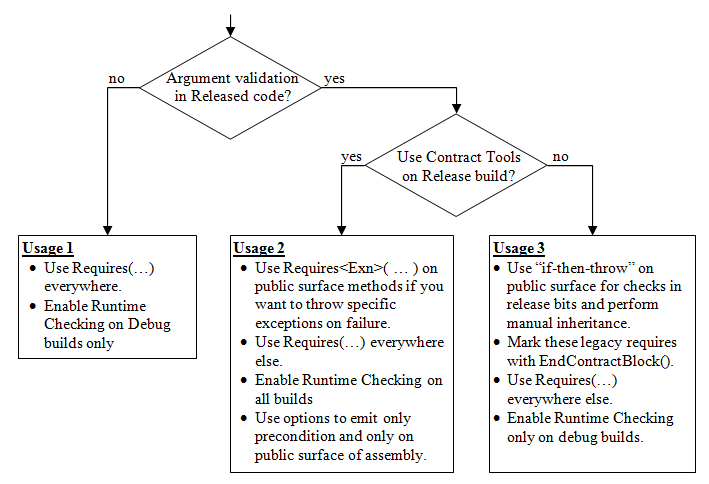
\includegraphics[width=\columnwidth]{UsageDecision.png}
\end{center}
  \caption{How to Perform Argument Validation}
  \label{fig:usagedecision}
\end{figure}

The easiest use of the contract tools is if you decide that you don't
need to perform argument validation at runtime in release builds
(Usage 1). In that case, you use the contract tools during
development, but not on the shipped bits. Remember, you can ship a
contract reference assembly along with your release bits so clients
can get runtime checking of your parameter validations on their debug
builds via call-site requires checking. 

The second easiest approach if you need argument validation in your
release build is to turn on contract checking in all builds (Usage
2). You therefore take advantage of the tools to produce the runtime
strings of your conditions and to perform contract inheritance for
you. You can choose to produce specific exceptions for your parameter
validations, or have the default ContractException. The risk of using
the contract tools in your release build is that you depend on tools
that have not reached production quality level. 

The trickiest combination is when you want argument validation in
release builds, but you are using the contract tool for runtime
checking only in debug builds, but not in the release build (Usage
3). In that case, you have to continue writing your argument
validation the way you already do, namely using if-then-throw
statements (we call them legacy-requires). If you want these to be
tool discoverable, add other contracts (such as Ensures) after them,
or use Contract.EndContractBlock(), if no other contracts are
present. Note that since you are not using the runtime checking tools
in the release build, you are not going to get any inheritance of
contracts and you have to manually repeat your legacy-requires on
overrides and interface implementations. For interface and abstract
methods, you still get the most benefit if you write contract classes
with normal requires and ensures forms so you get checking in your
debug builds and they appear in contract reference assemblies and are
thus visible to dependent projects and to static checkers.

\subsubsection{Assembly Mode}
\label{sec:assemblymode}
The contract tools need to know which usage mode you choose. If you
use VisualStudio, select the \textsf{Assemby Mode} on the contract
property pane as follows:
\begin{itemize}
\item Usage 1 or 2: Standard Contract Requires
\item Usage 3: Custom Parameter Validation
\end{itemize}
This permits the tools to emit proper warnings when you violate the
usage guidelines.
If you use the tools from the command-line, pass the proper argument
for the \textsf{-assemblyMode} option.

\subsubsection{Difference between \requiresn{Exn} and if-then-throw}
The difference between these two forms is whether we rely on tools to
perform inheritance of contracts or whether programmers manually
inherit them as in existing practice. \requires{Exn}(...) is intended to
be used with tool support, meaning that they are inherited in all
builds and the message strings are generated automatically to include
the failing condition. Well-formedness checks of contracts do not
allow specifying \requires{Exn} on overrides or interface
implementations.

On the other hand, legacy-requires (if-then-throw) try to capture
existing practice for release builds, while providing some extra
support for Debug builds using the tools. In Debug builds with
contract tool support, on failure of legacy-requires
the contract failure hook is called. This provides the ability to
detect otherwise silent failures (due to catches) in debug builds. 

\subsubsection{Forcing Projects to build with Contracts}
If you are using scenario 2 (\requiresn{Exn}) and you make your source
code available to other developers, you might want to alert them that
they need to use the tools to build your source. If so, you can insert
the following snippet into your project file at the end (after the
import of the CSharp or VisualBasic targets):
\begin{lstlisting}[language=XML,mathescape=false]
  <PropertyGroup>
    <CompileDependsOn>$(CompileDependsOn);CheckForCodeContracts</CompileDependsOn>
  </PropertyGroup>
  <Target Name="CheckForCodeContracts"
     Condition="'$(CodeContractsImported)' != 'true'">
     <Error Text="Project requires Code Contracts http://msdn.microsoft.com/en-us/devlabs/dd491992.aspx"/>
  </Target>
\end{lstlisting}

\subsection{Migrating Projects towards Contracts}
\label{sec:migration}
Likely, you have an existing project and you would like to start using
contracts with minimal changes. If after reading
Section~\ref{sec:usage} you determine that your project falls into
usage mode 1 or 2, you don't really have a migration task to do. This
section thus assumes that your project falls into usage 3, namely that it
contains explicit parameter validation code throwing exceptions, that
you want to ship such validation code in your release, and that the
contract rewriting tool will \emph{not} be used in your release build.

The goal of migration is to mark your existing argument validation
code so that the contract tools can recognize it. Once you have made
your validations recognizable, you can start to take advantage of the
tools as follows:
\begin{itemize}
\item You can use documentation generation to augment doc-xml files
  with contracts and produce documentation that includes explicit
  descriptions of your preconditions and other contracts (Section~\ref{sec:docgen}).
\item In your test/debug builds, you can enable the runtime contract
  checker to find inconsistencies in your
validation code (e.g., forgetting to validate parameters in overrides
or interface implementations)
\end{itemize}

\subsubsection{Marking Existing Validation Code as Contracts}
In methods containing argument validation code in the form of
\code{if-then-throw} statements, you should place a
\code{Contract.EndContractBlock()} call after the last such
statement as described in Section~\ref{sec:legacythrows}.

If your code uses helper methods to validate contracts, mark these methods
with a \code{ContractArgumentValidator} attribute as described in
Section~\ref{sec:contractargumentvalidators}.

\subsubsection{Issues with Early Return}
Sometimes, you have existing code as follows:
\begin{lstlisting}
  void MyMethod(string data) {
    if (data == null) return;
    if (data.Length == 0) throw new ArgumentException(...);
    ...
\end{lstlisting}
If you add an \code{EndContractBlock()} marker after the if-then-throw
statement, the contract tools will complain about the return statement
found in the contract section. In order to fix this, you have to move
the return after the parameter validation check, while at the same
time weakening the parameter validation to allow for \code{data} to be \code{null}:
\begin{lstlisting}
  void MyMethod(string data) {
    if (data != null && data.Length == 0) throw new ArgumentException(...);
    Contract.EndContractBlock();
    if (data == null) return;
    ...
\end{lstlisting}
This transformation makes the effective precondition explicit, which is
that either \code{data} is null, or \code{data.Length} is greater than
0: \code{Contract.Requires<ArgumentException>(data == null || data.Length > 0)}.


\subsubsection{Delegating Checks to Other Methods}
Suppose you have a code pattern similar to the following code:
\begin{lstlisting}
public class Base {
  public virtual void Compute(string data) {
    if (data == null) throw new ArgumentNullException(...);
    Contract.EndContractBlock();
    ...
  }
}

public class Derived : Base {
  public override void Compute(string data) {
    base.Compute(data);
    ...
  }
}
\end{lstlisting}
Then the tools will issue warning \code{CC1055} with a message of the form:
\begin{quote}
Method 'Derived.Compute' should contain custom argument validation for \\
'\requires{ArgumentNullException}\code{(data != null)}' as it overrides
'Base.Compute' which suggests it does.
\end{quote}
In this situation, the warning is not helpful, as the implementation
of \code{Derived.Compute} delegates the parameter validation to
another method (in this case the base method). To avoid the warning in
this situation without repeating the validation, you can add a
\code{SuppressMessage} attribute to the method:
\begin{lstlisting}
public class Derived : Base {
  [SuppressMessage("Microsoft.Contracts", "CC1055", Justification="Validation performed in base method")]
  public override void Compute(string data) {
    base.Compute(data);
    ...
  }
}
\end{lstlisting}


\subsubsection{Writing Interface Contracts}
You can specify interface contracts as explained in
Section~\ref{sec:interfacecontracts}. On interfaces you don't need to
use the if-then-throw form of contracts, as they are never executed
directly. Instead, you can use
\requires{Exception}\code{(...)} on interfaces. In builds where you
enable the tools, they make sure
that each implementation of the interface has validation code (Note:
the tools currently don't check that the validation code is equivalent, only
that you have any validation at all).

If you use \code{Requires(...)} on interface methods, these
preconditions will be enforced at runtime only in builds where you
enable runtime checking. Unlike for \requires{Exception}\code{(...)},
the inheritance of \code{Requires(...)} onto each implementation is
done by the tools and you don't need to repeat them.

\subsubsection{Going Further}
When you get to the point that you have marked existing validation as
contracts, and you get a clean build and test run of a debug build
with runtime checking enabled, you are ready to write more contracts
that are enforced in your debug/test runs. 

You can add invariant methods to enforce data
integrity (Section~\ref{sec:invariants}) and you can write
\code{Contract.Requires} for additional preconditions (Section~\ref{sec:preconditions}) and
\code{Contract.Ensures} for postconditions
(Section~\ref{sec:ensures}). These checks are enforced in your
testing builds with runtime checking enabled, but disappear from your shipping code.

Once you feel comfortable writing contracts and understand what they
do, you may want to start using the static contract checker. Please
read Section~\ref{sec:staticchecker} before embarking on this adventure.

\subsection{Contract Ordering}
Method contracts should be written with the different elements ordered
as follows:

\vspace*{5pt}
\begin{tabular}{|l|p{4in}|}
\hline
If-then-throw	& Backward-compatible public preconditions
\\
\hline
Requires, \requiresn{E} & All public preconditions
\\
\hline
Ensures & All public (normal) postconditions
\\
\hline
EnsuresOnThrow	& All public exceptional postconditions
\\
\hline
Ensures & All private/internal (normal) postconditions
\\
\hline
EnsuresOnThrow	& All private/internal exceptional postconditions
\\
\hline
EndContractBlock & If using if-then-throw-style preconditions without
any other contracts, place a call to \code{EndContractBlock} to
indicate all previous if checks are preconditions.
\\
\hline
\end{tabular}
\vspace*{5pt}

\subsection{Purity}
\label{sec:purity}
All methods called within a contract must be pure: that is, they must
not update any pre-existing state. (A pure method is allowed to modify
objects that have been created after entry into the pure method.)
Code Contract tools currently assume the following things are pure:
\begin{itemize}
\item	Methods marked \code{[Pure]} (If a type is marked \code{[Pure]}, then that applies to all of its methods.) The pure attribute is defined in the contract library. (Section~\ref{sec:pureattribute})
\item	Property getters.
\item	Operators (static methods whose names start with \code{op_}, have one or two parameters and a non-void return type).
\item	Any method whose fully qualified name begins with
  \code{System.Diagnostics.Contracts.Contract},
  \code{System.String}, \code{System.IO.Path}, or \code{System.Type}.
\item Any invoked delegate, provided that the delegate type itself is
  attributed with \code{[Pure]}. The existing delegate types
  \code{System.Predicate<T>} and \code{System.Comparison<T>} are
  considered pure.
\end{itemize}
In the future, there will be a purity checker that will enforce these assumptions.

\subsection{Visibility}
\label{sec:visibility}
All members mentioned in a contract must be at least as visible as the
method in which they appear. For instance, a private field cannot be
mentioned in a precondition for a public method: clients wouldn't be
able to validate such a contract before they call the method. However,
if the field is marked with the ContractPublicPropertyName attribute
(Section~\ref{sec:contractpublicattribute}), then it is exempt from these rules.

\subsection{Special Method Usage}
Special methods such as \code{Contract.Result<T>} can only appear
in \code{Ensures} contracts and type \code{T} must agree with the
method return type.



\begin{figure}[tb!]
\begin{center}
  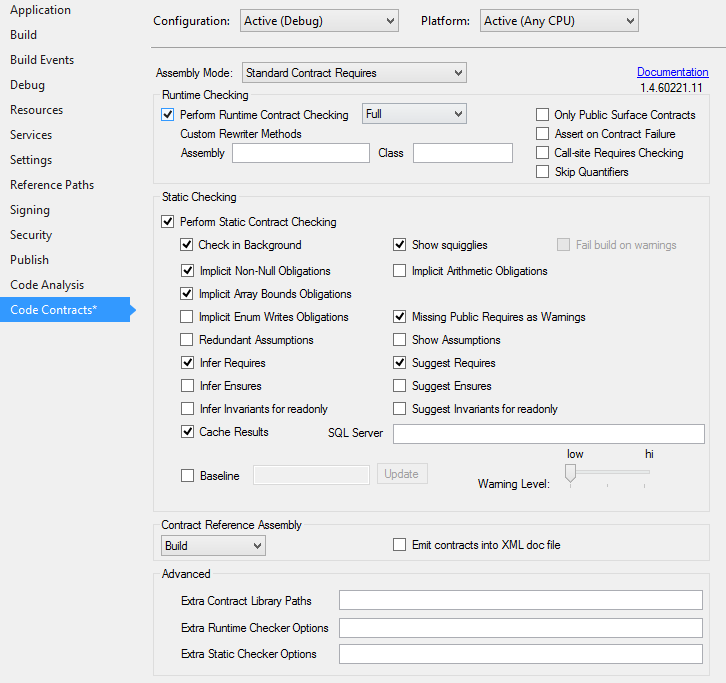
\includegraphics[width=.8\columnwidth]{VSUI1.png}
\end{center}
  \caption{Contract Property Pane in Visual Studio}
  \label{fig:property-pane}
\end{figure}

\section{Visual Studio Integration}
\label{sec:vsintegration}
When the managed contracts plugin is installed, \csharp{} and VB projects
within Visual Studio are augmented with an extra property pane
entitled ``Code Contracts", as shown in Figure~\ref{fig:property-pane}. This pane provides
configuration specific options for enabling runtime contract checking,
as well as static contract checking.

If you are using contracts with a target platform of 4.0 or later and
you are referencing (implicitly) mscorlib.dll, then the
\code{Contract} class appears in the
\code{System.Diagnostics.Contracts} namespace. If you are using a
pre-4.0 target platform, you need to add a reference to the
\code{Microsoft.Contracts.dll} library. The library should appear
under the .NET tab when adding project references.

\subsection{Assembly Mode}
Use the assembly mode selection on the UI to indicate to the tools
what usage mode (Section~\ref{sec:usage}) you want for the
present project:
\subsubsection{Custom Parameter Validation}
Select this mode if your project falls into usage 3
(Section~\ref{sec:usage}), i.e., you want to check parameter validation in your
released version of the code \emph{and} you \emph{don't run the
contract rewriter} on your release bits.

In this mode, you can use legacy if-then-throw statements and
\textsf{[ContractArgumentValidator]} methods to express parameter
validation code that you want the contract tools to recognize. 
You have to manually perform inheritance of such validation code and
the tools warn you if it sees overrides/implementations where such
validation appears to be missing.
You can use ordinary \textsf{Requires(condition)} for debug only
preconditions. These will be inherited automatically, but only appear
in builds where you enable the contract rewriter.

In this mode, you are not allowed to use the \requires{Exn} form,
except on contract classes for interfaces and abstract types. If you do,
the tools will issue an error.

\subsubsection{Standard Contract Requires}
Select this mode if your project falls into usage 1 or 2
(Section~\ref{sec:usage}), i.e., you either don't want parameter
validation in your released code, or you run the contract rewriter on
your released code.

In this mode, you are not allowed to use legacy if-then-throw blocks
marked as contracts with \code{EndContractBlock} or
\code{[ContractArgumentValidator]} methods. The tools will emit errors
if you do.

\subsection{Runtime Contract Checking}
We suggest using either a standard \code{Debug} (or Checked)
configuration or a custom configuration to use runtime contract
checking. The benefit of a custom configuration is to allow separate
testing of potentially expensive contract checks without affecting
existing test runs with stricter timing constraints.

To enable runtime contract checking in a particular configuration,
select the configuration and check the box for runtime contract
checking. We also recommend you select \textbf{Build} to build a contract reference assembly 
(see Section~\ref{sec:contractreferenceassemblies}).

\subsubsection{Runtime Checking Level}
 The drop-down menu to the right let's you select the level
of runtime contract checking. The enabled contract checks depending on
the level are listed in the
table below:
\begin{center}
\begin{tabular}{|l|c|c|c|c|c|c|c|}
\hline
& \multicolumn{7}{|c|}{Enabled Runtime Checks} \\
Checking Level & Legacy & \requiresn{E} & Requires & Ensures & Invariants & Asserts & Assumes
\\
\hline
\hline
Full           & X      & X              & X        & X       & X          & X\footnotemark[1]       & X\footnotemark[1]
\\
\hline
Pre and Post   & X      & X              & X        & X       &            &         &
\\
\hline
Preconditions  & X      & X              & X        &         &            &         &
\\
\hline
ReleaseRequires & X      & X              &          &         &            &         &
\\
\hline
None           &        &                &          &         &            &         &
\\
\hline
\end{tabular}
\footnotetext[1]{These are omitted if \emph{Only Public Surface Contracts} is enabled.}
\end{center}

\noindent By ``Legacy'', we mean any if-then-throw blocks preceding any
\code{Contract.*} methods, which are therefore recognized as
declarations of preconditions.

Note that when level ``None'' is selected, all contracts are erased,
including ``Legacy requires''. This level is useful mainly for
doing benchmarking without any contracts.


\subsubsection{Public Surface Contract Checks}
In addition to the level, the checkbox \emph{Only Public Surface
  Contracts} can be used to erase all contracts on methods that are
not callable from outside the assembly (even via interfaces). In
addition, all \code{Assume} and \code{Assert} contracts in all methods
are erased.

\textbf{Warning}: if you create a delegate from a method that is not
visible from outside the assembly and the delegate itself will be
callable from outside the assembly, then any parameter validation on
this method will not trigger with this box checked.

\textbf{Warning}: if you \emph{delay} parameter validation on a method callable
from outside by having it call a method not callable from outside the
assembly that performs the validation, then you will get \emph{no
validation} with this box checked, as the validation on the
non-visible method is erased.

\subsubsection{Assert on Contract Failure}
\noindent
When this box is checked (default), all contract failures, including
\requires{E} and legacy requires (marked if-then-throws) trigger the
default failure behavior of the contract library, which is to display
an assert dialog. Clearing this box will instead generate code that throws
exceptions on failure. See Section~\ref{sec:runtimecontractbehavior}
for details.

\subsubsection{Call-site Requires Checking}
When building a project $A$ with call-site requires checking on, the
rewriter will determine at each call-site within $A$ if the call
``potentially'' calls a method defined in another assembly. In that
case, the rewriter will insert the \code{Requires} checks for the
called method at the call-site within assembly $A$ (actually, we use
wrapper methods to avoid duplicating the checks). Of course, in order
for this to work, the contracts for the called method need to be
known, which will require contract reference assemblies ($B$.\code{Contracts},
if the method is defined in assembly $B$).

\noindent Some \code{Requires} checks are not currently instrumented at
call-sites:
\begin{itemize}
\item Requires of constructors
\item Requires of protected methods
\end{itemize}

\noindent
Call-site requires checking enables a library writer to
produce a library $B$ without runtime \code{Requires} checks (e.g.,
for performance reasons), while providing the \code{Requires}
separately in a contract reference assembly $B$.\code{Contracts}. A
developer of a project $A$ referencing $B$ and using call-site
requires checking will have parameter validations checked for methods
in $B$, regardless of whether $B$ is actually instrumented with checks
or not.

\subsubsection{Skip Quantifiers}
Quantifier checking can be expensive at runtime as it may traverse
large collections of data. Enabling skip quantifiers will skip any
contracts that contain \code{Contract.ForAll} or
\code{Contract.Exists} calls.

\subsubsection{Build Steps}
\noindent
When runtime contract checking is enabled, a build will perform the
following actions in addition to the regular compile:
\begin{itemize}
\item It determines the availablility of contract reference assemblies
  for all referenced projects and warns if they are missing (Section~\ref{sec:contractreferenceassemblies}).
\item It applies the contract rewriter \code{ccrewrite} to the target assembly, performing well-formedness checks on the contracts, instrumenting contract runtime checks into the appropriate places, including contract inheritance (Section~\ref{sec:runtimecontractchecking}).
\end{itemize}

\subsubsection{Extra Options}
The boxes labeled \textit{custom rewriter methods} can be used to
customize the runtime behavior for contract failure by specifying an
assembly (relative to the project output directory) and the full
namespace path to the type containing the custom failure behavior (see
Section~\ref{sec:runtimecontractbehavior}). The specified assembly may
be the project output itself.

Under the \textit{advanced} options, extra library paths (semi-colon
separated) can be specified for finding contract reference
assemblies. Extra runtime checker and static checker command line options can be
specified there as well.

\subsubsection{Suppressing Warnings}
\label{sec:suppresswarnings}
You can suppress warnings you get from the tools by adding
\code{SuppressMessage} attributes to methods. For example,
to suppress a warning \code{CC1055} about missing validation on a
method, add the following attribute:
\begin{lstlisting}
[SuppressMessage("Microsoft.Contracts", "CC1055", Justification="Check performed in DelegateTo")] 
public override void Compute(string s) {
  DelegateTo(s);
}
\end{lstlisting}
In general, to suppress any warning, use the above pattern with the
appropriate error number you want to suppress. The error number should
be visible in the output window if it is not included in the message
on the Error List window.

You can place \code{SuppressMessage} attributes on types and
properties in addition to methods. In that case, the suppression
applies to the entire scope of the type or property.

\subsection{C\# Code Snippets}

The installer adds a number of \csharp{} code snippets that are useful
for authoring code contracts. Each snippet in the table below is
invoked by typing the character shortcut and hitting TAB TAB (tab
twice).
\begin{center}
\codefamily
\begin{tabular}{|l|l|}
\hline
Shortcut & Contract Snippet \\
\hline
\hline
cr & Contract.Requires(...);
\\
\hline
ce & Contract.Ensures(...);
\\
\hline
ci & Contract.Invariant(...);
\\
\hline
crr & Contract.Result$\langle$...$\rangle$()
\\
\hline
co & Contract.OldValue(...)
\\
\hline
cim & \multicolumn{1}{p{6cm}|}{
\raggedright
[ContractInvariantMethod]\linebreak
private ObjectInvariant() \{ \linebreak
\hspace*{5mm} Contract.Invariant(...); \linebreak
\}}
\\
\hline
crn & Contract.Requires(... != null);
\\
\hline
cen & Contract.Ensures(Contracts.Result$\langle$...$\rangle$() != null);
\\
\hline
crsn & Contract.Requires( !String.IsNullOrEmpty(...) );
\\
\hline
cesn & Contract.Ensures( !String.IsNullOrEmpty(Contracts.Result$\langle$string$\rangle$()) );
\\
\hline
cca & Contract.Assert(...);
\\
\hline
cam & Contract.Assume(...);
\\
\hline
cre & Contract.\requiresn{E}(...);
\\
\hline
cren & Contract.\requires{ArgumentNullException}(... != null);
\\
\hline
cresn & Contract.\requires{ArgumentException}( !String.IsNullOrEmpty(...) );
\\
\hline
cintf & expands to an interface template and associated contract class
\\
\hline
\end{tabular}
\end{center}



\subsection{VB Code Snippets}

The installer also adds Visual Basic code snippets similar to the ones for \csharp{}.
Each snippet in the table below is
invoked by typing the shortcut and hitting TAB (tab once).
\begin{center}
\codefamily
\begin{tabular}{|l|l|}
\hline
Shortcut & Contract Snippet \\
\hline
\hline
creq & Contract.Requires(...)
\\
\hline
cens & Contract.Ensures(...)
\\
\hline
cinv & Contract.Invariant(...)
\\
\hline
crr & Contract.Result(Of ...)()
\\
\hline
cold & Contract.OldValue(...)
\\
\hline
cim & \multicolumn{1}{p{6cm}|}{
\raggedright
$\langle$ContractInvariantMethod()$\rangle$ \_\linebreak
Private Sub ObjectInvariant() \linebreak
\hspace*{5mm} Contract.Invariant(...) \linebreak
End Sub}
\\
\hline
crn & Contract.Requires(... IsNot Nothing)
\\
\hline
cen & Contract.Ensures(Contracts.Result(Of ...)() IsNot Nothing)
\\
\hline
crsn & Contract.Requires( Not String.IsNullOrEmpty(...) )
\\
\hline
cesn & Contract.Ensures( Not String.IsNullOrEmpty(Contracts.Result(Of string)()) )
\\
\hline
cca & Contract.Assert(...)
\\
\hline
cam & Contract.Assume(...)
\\
\hline
cre & Contract.Requires(Of Exc)(...)
\\
\hline
cren & Contract.Requires(Of ArgumentNullException)(... NotIs Nothing)
\\
\hline
cresn & Contract.Requires(Of ArgumentException)( Not String.IsNullOrEmpty(...) )
\\
\hline
cintf & expands to an interface template and associated contract class
\\
\hline
\end{tabular}
\end{center}

\subsection{Building a Contract Reference Assembly}
\label{sec:contractreferenceassemblies}
\emph{Note change from previous behavior: Contract reference
  assemblies are not longer built automatically for all
  dependee projects of a project.}

If your project contains contracts and is referenced by other
projects, we strongly recommend that you select \textbf{Build} under
the contract reference assemby section in the properties tab for
CodeContracts. 

The contract reference assembly for an assembly named \code{A} will be
called \code{A.Contracts.dll} and appears in the project output
directory. It can be distributed along with your assembly so other
developers can take advantage of the contracts for your project.

This contract reference assembly is crucial to make the contracts in
your project available to referencing projects. Without building a
contract reference assembly, other projects cannot determine what
contracts are present.

The drop down for building contract reference assemblies has three
selections: (none), Build, and DoNotBuild. The behavior of these
selections is described below:
\begin{itemize}
\item \textbf{(none)}: this is the default setting when you haven't
  made an explicit choice yet. If another project requires the
  contracts of this project, the build will warn you that no contract
  reference assembly was found. To get rid of this build warning,
  select either \textbf{Build} or \textbf{DoNotBuild}.

\item \textbf{Build}: this is the recommended setting when your
  project has contracts. It will produce
  an assembly called \code{A.Contracts.dll} in the output directory of
  project \code{A}. It makes the contracts of \code{A} visible to
  other projects.

\item \textbf{DoNotBuild}: this setting is recommended if this project
  does not contain contracts, or there are problems building the
  contract reference assembly. With this setting, the build warning
  about missing the contract reference assembly produced when other
  projects reference this project will disappear.
\end{itemize}

\noindent
For a description of the command line tool to build contract reference
assemblies, see
Section~\ref{sec:contractreferenceassemblies-appendix}.

\subsection{Static Contract Checking}
\label{sec:staticchecker}
First, a word of caution: Static code checking or verification is a
difficult endeavor. It requires a relatively large effort in terms of
writing contracts, determining why a particular property cannot be
proven, and finding a way to help the checker see the light.

Before you start using the static contract checker in earnest, we
suggest you spend enough time using contracts for runtime checking to
familiarize yourself with contracts and the benefits they bring in
that domain.

\subsubsection{Current Limitations of the Checker and Bugs}
Below is a list of known bugs or unimplemented features in the static
contract checker:
\paragraph{Known Limitations}
\begin{itemize}
\item Invariants are only checked by the static checker on method
  exits, but not prior to calls. It is thus easy to trick the checker
  into thinking the invariant on \code{this} holds by calling an empty
  method on \code{this}.

\item Invariants on structs are checked the same way as invariants on
  classes. However, since structs always have an implicit emtpy default
  constructor, and this constructor is not checked, invariants
  violated by the default constructor are not reported.

\item The static contract checker has limited supported for
  \code{ForAll} and \code{Exists} quantifiers, provided the quantified expression is
  simple like \code{x => x != null}.

\item when writing iterators using 
  \code{yield}, the static contract checker will not be able to
  prove postconditions (see Section~\ref{sec:iterators}).

\item post conditions of async methods are not checked by the static checker.
\end{itemize}



\subsubsection{Setting Up a Configuration}
If you are still determined to go ahead with contracts, we suggest you
create a separate configuration, e.g., CodeAnalysis---based on your
Debug configuration---and enable static checking for that
configuration. This avoids slowing down regular build flavors. 

To enable static checking, check the box titled \textit{Perform Static
Contract Checking}. If static checking is enabled, a build performs
the following steps:
\begin{itemize}
\item It builds an alternate target for the project with
\code{CONTRACTS_FULL} symbol defined. The target is called
\code{X.decl.dll} where \code{X} is the regular assembly name of the
project.
\item It runs the static verifier on \code{X.decl.dll} and displays warnings in the output and task windows.
\end{itemize}

\subsubsection{Static Checking Options}
\label{sec:staticcheckingoptions}
By default, the static verification tries to prove all explicit
contracts in the code under analysis (assertions, invariants,
requires, and ensures), as well as requires of methods called in other
assemblies, and inherited ensures and object invariants on classes
extending base classes and interfaces in other assemblies.

\paragraph{Check in Background:} This option (on by default) controls
whether the running of the static checker will block your
build.

\paragraph{Show squigglies:} Controls whether warnings emitted by the
static checker appear as squigglies in the source text. It is off by
default as the squigglies can be overwhelming if lots of warnings are
emitted.

\paragraph{Cache results:} Controls if the analysis results are
cached. If checked, the analysis tries to avoid analyzing methods
whose outcomes cannot possibly change (because no contracts, no code,
and no relevant metdata has changed). Enabling this option allows for
faster turn-around times if using the static checker repeatedly.

To share the cache among multiple developers, use a SQL server and put
the server name in the SQL Server configuration box in the UI. Note:
the SQL server connection uses Windows authentication to log onto the
server. Your developers will need the right to create and modify
databases.

If you see connection timeouts, you can increase the timeout by adding
\[
\mathtt{-cacheserverTimeout}\ \textit{value}   
\]
in the extra static checker options.


\paragraph{Implicit obligations:}
The check box \emph{Implicit Non-Null Obligations} enables additional
checks, which warn about potential inappropriate uses of null in the code
under analysis.
Similarly, the check box \emph{Implicit Array Bounds Obligations}
causes the verifier to try to validate the following:
\begin{itemize}
\item Array accesses are within bounds of the array (lower and upper).
\item Array creation uses a non-negative size.
\end{itemize}
Enabling \emph{Implicit Arithmetic Obligations} causes the checker to
warn about division by zero errors, 
floating point precision mismatches, and erroneous negations of
\code{Int.MinValue}.
The \emph{Implicit Enum Writes Obligations} checks that when a value is written into a location of enum type, the value is one of the defined values for such a type.

We suggest you do \emph{not} enable the implicit checks initially, as
they easily lead to too many warnings if you enable the checking on an
existing code base. For a new code base, feel free to enable them
initially.

\paragraph{Redundant Assumptions:} Enabling this option causes the
checker to attempt to prove the \code{Contract.Assume} statements 
and warn if they are provable. We suggest you use this option only
occasionally to get rid of redundant assumptions, but not on a
continuous basis, as it slows down the static analysis substantially.


\paragraph{Show Assumptions:}
This options let the static checker making explicit some of the implicit assumptions you made in your code.
Examples are assumptions on the value returned by a method, on the input parameters or object fields that cannot be expressed by preconditions because they violate visibility rules.

\paragraph{Missing Public Requires}
When this option is selected, the static checker will warn about
missing requires on methods visible outside the assembly. Effectively,
the option turns suggested requires on such methods into warnings.

\subsubsection{Inference}
\label{sec:Inference}
The static checker helps the annotation process by suggesting contracts, and propagating them to the callers.
The first time you run inference, it may take some time, so please be patient.
We suggest to use inference together with caching.
The ``infer'' switches  propagate the inferred contracts to the callers.
The ``suggest'' switches simply print out the inferred contracts in the output window.
The static checker infers/suggest preconditions from failing assertions.
The suggested/inferred preconditions are necessary in that, if they do not hold then the method is doomed to fail.
By default, the static checker filters preconditions containing disjunctions. 
To enable them, check the ``disjunctive requires'' box.
The static checker uses some heuristics to derive to filter the method postconditions inferred/suggested to the user.
Object invariants are inferred/suggested from the failing assertions involving readonly fields.

\subsubsection{Caching of the Analysis Results}
\label{sec:caching}
By default, after a build, the static verifier analyzes all the methods in a given assembly.
However, it is often the case that only few methods changed among two builds.
The caching mechanism allows to persist the analysis results between builds and it avoids re-analyzing most of the unmodified methods. 
To activate it, simply check the box in the Visual Studio pane.

\subsubsection{Focus Your Attention}
As mentioned in the introduction, static verification is difficult and
at times overwhelming. To not get lost in a sea of warnings, we
suggest you focus the static contract checker on a small part of your code and
drill down in that area. To do so, use the attribute
\begin{lstlisting}
[assembly:ContractVerification(false)]
\end{lstlisting}
in your assembly. This attribute at the assembly level turns off
contract checking by default. Now you can focus the static contract checker on
individual methods or individual types by adding the attribute
\begin{lstlisting}
[ContractVerification(true)]
\end{lstlisting}
to a class, struct, or individual method. The attribute changes the
default for the sub-tree of code it appears on. This means you can
switch the default mutliple times, e.g., if enabled on a particular
type, you can disable it again for a
nested class or individual methods.

Once you are happy with the contract checking in the small set of methods you
focused on, you can grow the set incrementally. Note that you may need
to write contracts on methods \emph{called} from your set of checked
methods, even if the called methods themselves are not in your focus
set.


\subsubsection{Dealing with Warnings}
When the static verifier issues a warning about a particular contract
or implicit proof obligation, it doesn't necessarily indicate an error
in the code. Warnings are issued whenever the checker is \emph{unable
to prove} that the contract holds on all executions under the
assumptions provided by the contracts on all other methods. 

If the verifier emits a warning that the programmer deems unwarranted,
it is possible for the programmer to make this explicit in a number of
ways. Most often, it is possible to add a requires to the method where
the warning occurs to make some assumption between callers and the
method explicit. For example, if the method uses a parameter \code{p} without checking for null, the method wants to assume that callers never pass null. In order for the verifier to understand this, add a precondition of the form:
\begin{lstlisting}
Contract.Requires( p != null );
\end{lstlisting}
If the warnings concerns internal object state of fields that might
not be visible to all callers of the method, then this might indicate
the need for an object invariant. For example, if a field \code{f} is
assumed to be non-null at all times, an object invariant should be
added:
\begin{lstlisting}
[InvariantMethod]
private void ObjectInvariant() {
  Contract.Invariant( f != null );
}
\end{lstlisting}
This invariant is now assumed on all method entries of this class, and
it is checked on all method exits, and in addition on exit of all
constructors.

Alternatively, it might be that the method where the warning is
emitted obtains a value as a result from a call to another method
\code{M} and uses it without checking for null. Again, the method
assumes that the result of \code{M} is non-null given the particular
parameters. This can be made explicit by adding a contract to \code{M}
of the form:
\begin{lstlisting}
Contract.Ensures( Contract.Result<T>() != null );
\end{lstlisting}
where \code{T} is the return type of \code{M}. If the method returns
non-null only provided certain properties hold of the parameters, that
can be made explicit as well by using a disjunction in the
ensures. For example, method \code{M} might return null if a parameter
\code{p} is null, otherwise it returns non-null. This is expressed
as follows:
\begin{lstlisting}
Contract.Ensures( p == null || Contract.Result<T>() != null );
\end{lstlisting}
Another way to read the above disjunction is as an implication: \code{p != null ==> result != null}.

For some warnings it will either be too complicated to add all the
invariants to the code to show why a particular contract should be
true, or the verifier might have inherent limitations that prevent it
from proving it. In cases where all else fails, it is always possible
to add an explicit assumption in the code. For example, if some local
\code{x} is known to be non-null at a given program point, but there
is no other way to teach the verifier why this is so, then an explicit
\code{Assume} statement will do the trick:
\begin{lstlisting}
Contract.Assume( x != null );
\end{lstlisting}
Such assumptions are silently believed by the static
verification. However, they are still checked at runtime when using
runtime checks. Thus, accidental erroneous assumptions added by
programmers can be discovered during testing.

\subsubsection{Baseline}
Bringing an existing code base to a point where the verifier emits
only a few warnings is difficult and time consuming, as it requires
adding numerous contracts. To make it easier to use contracts on
existing code bases, and to focus warnings introduced by new code or
code changes, the \emph{Baseline} functionality can be used.

To use the baseline functionality, check the box labelled
\emph{Baseline} and provide a file name to store the baseline in. The
path is relative to the project output directory.  When the analysis
is run and the baseline file does not exist, the baseline is
created. During this run, all warnings are shown in the output and
stored in the baseline file as XML.

When the analysis is run and the baseline file exists, then the
baseline acts as a filter and warnings already found in the baseline
are not shown again. New warnings are shown and stored in a file
called \code{\<baseline\>.new}, where \code{\<baseline\>} is the file
name of the baseline file. Since the files are stored as textual XML,
it is possible to edit them and to add additional failures to the baseline.
The format does not depend on method ordering and additional XML tags
for grouping can be introduced freely.

\subsubsection{Relevant Warnings}
\label{sec:relevantWarnings}
The \emph{Warning Level} slider enables a heuristic to report the most relevant warnings. 
By default, it is set to Low, i.e., only the most relevant warnings are reported in the Error List window. 


\subsubsection{Filtering Warning Messages}
\label{sec:filteringstaticcheckerwarnings}

If using \code{Contract.Assume} is ineffective to quiet noise in the
static contract checker warnings, a last resort is to turn off certain warnings
using the CodeAnalysis \code{SuppressMessage} attribute.
To instruct the static contract checker not to emit a particular class of
warnings for a method (a type, an assembly), annotate the method (the
type, the assembly) with the attribute:
\begin{lstlisting}
[System.Diagnostics.CodeAnalysis.SuppressMessage("Microsoft.Contracts", warningFamily)]
\end{lstlisting}
where \code{warningFamily} is one of: \code{Requires}, \code{Ensures},
\code{Invariant}, \code{NonNull}, \code{ArrayCreation},
\code{ArrayLowerBound}, \code{ArrayUpperBound}, \code{DivByZero}, \code{MinValueNegation}.

If necessary, the static contract checker allows filtering a single warning message
(instead of an entire family) as well.
To do so you can annotate a method with the attribute
\begin{lstlisting}
[System.Diagnostics.CodeAnalysis.SuppressMessage("Microsoft.Contracts", warningFamily-ILOffset-MethodILOffset)]
\end{lstlisting}
where \code{warningFamily} is as above, and ILOffset and
MethodILOffset are used by the static contract checker to determine
the program point the warning refers to.
The offsets can be obtained from the static contract checker by providing the \code{-outputwarnmasks} switch in the
``Custom Options'' entry in the VS pane. Check the Build Output Window
for the necessary information. Code changes to the method or the
contract being violated may invalidate the IL offsets and turn the
suppression ineffective. 

Sometimes the precondition for a method may be too complex for the static analyzer.
In order to suppress all the warning messages issued at call sites, one can use the \code{RequiresAtCall} modifier:
\begin{lstlisting}
[System.Diagnostics.CodeAnalysis.SuppressMessage("Microsoft.Contracts", ``RequiresAtCall-exp'')]
\end{lstlisting}
where \code{exp} is a string describing the condition to be ignored.
The attribute should be added to the method where the precondition is defined. 
The \code{-outputwarnmasks} switch provides (in the Build Output Window) the necessary information.
The \code{EnsuresInMethod} modifier allows to suppress all the warnings related to  a postcondition   in all the methods implementing or overriding  the current method.
The attribute should be added to the method where the postcondition is defined.
The \code{InvariantInMethod} modifier allows to suppress all the warnings related to an object invariant.
The attribute should be added to the type where the invariants is defined.

\section{Runtime Contract Behavior}
\label{sec:runtimecontractbehavior}
\label{sec:runtimecontractchecking}

The runtime behavior of a contract can be configured at the time the
contract rewriter is run and also during program execution.

The basic operation of the contract rewriter is to place runtime
checks for contracts at appropriate places. The contracts may come
from a variety of places, e.g., via inheritance from contract
reference assemblies or other code in the assembly being rewritten. 


\subsection{Rewriter Methods}
Every contract usage is translated to call a particular rewriter
method according to the table below:
\begin{center}
\small
\begin{tabular}{|l|l|}
\hline
Requires(cond) & CR.Requires(cond, null, ``cond'') \\
\hline
Requires(cond, msg)&	CR.Requires(cond, msg, ``cond'') \\
\hline
\requiresn{E}(cond) & CR.\requiresn{E}(cond, null, ``cond'') \\
\hline
\requiresn{E}(cond, msg)&	CR.\requiresn{E}(cond, msg, ``cond'') \\
\hline
Ensures(cond)	& CR.Ensures(cond, null, ``cond'') \\
\hline
Ensures(cond,msg)	& CR.Ensures(cond, msg, ``cond'') \\
\hline
\EnsuresOnThrow{E}(cond)	& CR.EnsuresOnThrow(cond, null, ``cond'', exn) \\
\hline
\EnsuresOnThrow{E}(cond,msg)	& CR.EnsuresOnThrow(cond, msg, ``cond'', exn) \\
\hline
Invariant(cond)	& CR.Invariant(cond, null, ``cond'') \\
\hline
Invariant(cond, msg)	&CR.Invariant(cond, msg, ``cond'') \\
\hline
Assert(cond)	&CR.Assert(cond, null, ``cond'') \\
\hline
Assert(cond, msg)	& CR.Assert(cond, msg, ``cond'') \\
\hline
Assume(cond)	& CR.Assume(cond, null, ``cond'') \\
\hline
Assume(cond, msg)	& CR.Assume(cond, msg, ``cond'') \\
\hline
\end{tabular}
\end{center}

For legacy requires (if-then-throw), the rewriting
depends on a switch to the contract rewriter on whether to additionally assert on failure:
\begin{center}
\small
\begin{tabular}{|l|l|l|}
\hline
 & Assert on failure & Throw on failure (default) \\
\hline
(legacy require) if cond then throw &
\multicolumn{1}{p{2in}|}{\raggedright if cond then \{
  \hspace*{1em} var m = CR.RaiseContractFailedEvent(...);
  \hspace*{1em} if (m != null) Assert(false, m);
  \hspace*{1em} throw}
  &
\multicolumn{1}{p{2in}|}{\raggedright if cond then \{
  \hspace*{1em} CR.RaiseContractFailedEvent(...); \hspace*{1em} throw} \\
\hline
\end{tabular}
\end{center}

As you can see, the different overloads are all reduced to calls on 7
distinct methods in a contract runtime class \code{CR}:
\begin{lstlisting}
class CR {
  void Requires(bool cond, string userMessage, string condition);
  void Requires<E>(bool cond, string userMessage, string condition);
  void Ensures(bool cond, string userMessage, string condition);
  void EnsuresOnThrow(bool cond, string userMessage, string condition, Exception exn);
  void Invariant(bool cond, string userMessage, string condition);
  void Assert(bool cond, string userMessage, string condition);
  void Assume(bool cond, string userMessage, string condition);
}
\end{lstlisting}
The exception argument to \code{EnsuresOnThrow} is the actual caught
exception. These runtime contract methods are either generated by
the contract rewriter in the generated type
\code{System.Diagnostics.Contracts.\_\_ContractsRuntime}, or they can be
provided by the programmer as custom rewriter methods to the
contract rewriter (see Section~\ref{sec:customrewritermethods}). 

In the case where the contract rewriter synthesizes the methods, they all have the
following form:
\begin{lstlisting}
void Requires(bool cond, string userMessage, string condition) {
  if (cond) return;
  ReportFailure(ContractFailureKind.Precondition, userMessage, condition, null);
}
\end{lstlisting}
That is, the methods return if the condition is true. Otherwise, they
call \code{ReportFailure}. The other contract methods are
similar. \code{EnsuresOnThrow} passes the caught exception on to the
\code{ReportFailure} method.

The method that has special pre-defined failure behavior is
\requires{E}. It looks for a public constructor of the given exception type
that takes two string arguments. It then passes the message
constructed by user provided by \code{RaiseContractFailedEvent} and
the user provided message to the exception constructor. For the
standard \code{ArgumentException} type, the intention is that the
second parameter (the optional user provided message) is the parameter name.
Since \code{ArgumentNullException} takes these parameters in reversed
order, the generated code reverses the arguments in that case.
If no two argument constructor is found, constructor with a single
string argument is tried. If found, it is used to construct
the exception passing as a parameter the message constructed by
\code{RaiseContractFailedEvent}.
\begin{lstlisting}
void Requires<E>(bool cond, string userMessage, string condition)
  where E:Exception {
  if (cond) return;
  string str = TestRewriterMethods.RaiseContractFailedEvent(ContractFailureKind.Precondition, message, conditionText, null);
#if AssertOnFailure
  if (str != null) {
    System.Diagnostics.Debug.Assert(false, str);
  }
#endif
  Exception exception = null;
  ConstructorInfo constructor = typeof(TException).GetConstructor(new Type[] { typeof(string), typeof(string) });
  if (constructor != null)
  {
    if (constructor.GetParameters()[0].Name == "paramName")
    {
      exception = constructor.Invoke(new object[] { message, str }) as Exception;
    }
    else
    {
      exception = constructor.Invoke(new object[] { str, message }) as Exception;
    }
  }
  else
  {
    constructor = typeof(TException).GetConstructor(new Type[] { typeof(string) });
    if (constructor != null)
    {
      exception = constructor.Invoke(new object[] { str }) as Exception;
    }
  }
  if (exception == null)
  {
    throw new ArgumentException(str, message);
  }
  throw exception;
}
\end{lstlisting}
To use \code{Requires<E>} properly with \code{ArgumentNullException}
or \code{ArgumentOutOfRangeException}, use the second argument to
\code{Requires} to pass the parameter name:
\begin{lstlisting}
void TestMe(string name, int index) {
  Contract.Requires<ArgumentNullException>(name != null, "name");
  Contract.Requires<ArgumentOutOfRangeException>(index >= 0, "index");
\end{lstlisting}

\noindent The \code{ReportFailure} and \code{RaiseContractFailedEvent} methods are discussed
below.

\subsection{ReportFailure Method}
The \code{ReportFailure} method can be provided as part of the custom
runtime contract class (Section~\ref{sec:customrewritermethods}). Otherwise the following method
is synthesized: 
\begin{lstlisting}
void ReportFailure(ContractFailureKind kind, string userMessage,
                  string condition, Exception inner) 
{
  var message = RaiseContractFailedEvent(kind, userMessage, condition, inner);
  if (message == null) return; // handled
  TriggerFailure(kind, message, userMessage, condition, inner);
}
\end{lstlisting}
\code{ReportFailure} first calls the \code{RaiseContractFailedEvent} method which returns
either null if the failure is handled, or the message string to use
when calling \code{TriggerFailure}. 

The two methods called \code{RaiseContractFailedEvent} and
\code{TriggerFailure} can also be provided by the user in the supplied
custom runtime contract class
(Section~\ref{sec:customrewritermethods}). Otherwise, the methods from
the \code{Microsoft.Contracts.dll} or \code{mscorlib.dll} are used.

\subsection{RaiseContractFailedEvent}
The default implementation of \code{RaiseContractFailedEvent} in the library is to
call each handler registered with the \code{Contract.ContractFailed}
event. Exceptions thrown by handlers are ignored, but each handler can
indicate whether the failure is handled by calling \code{SetHandled()}
on the event argument. If any handler sets the failure as handled,
the method returns null and no further action is taken.

Alternatively, handlers can call \code{SetUnwind()} on the event argument to ask the code to
unwind. In that case, a \code{ContractException} is thrown after all
handlers have executed.

If a handler throws an exception, it is treated as if it called
\code{SetUnwind}. Additionally, the thrown exception will be used as
the inner exception of the \code{ContractException} thrown after all
handlers have executed. When multiple handlers throw, the inner
exception used is undetermined. 

\subsection{TriggerFailure}
The default implementation of \code{TriggerFailure} in the library is to
break into the debugger (if attached) or display an assert dialog
box. 

If the option ``assert on contract failure'' in the Visual Studio
Contract property pane is cleared, or the /throwonfailure option is
used on the command line, the contract rewriter instead synthesizes an
alternative \code{TriggerFailure} method that throws a
\code{ContractException}.  Note that the \code{ContractException} type
is added internally to the assembly being runtime checked.

\subsection{Rationale for Runtime Behavior}

Why, you might ask, is the runtime behavior for contract failure not
just to throw an exception?

A lot of discussion has gone into the
current design in order to address the following problem with
exceptions: \emph{thrown exception can be handled}. This means that in
your debugging or test runs, you might actually fail some contracts,
but the exception being thrown gets caught and silently swallowed
somewhere and nothing ever gets reported about the contract
failure. This is particularly annoying in the case where in your
Release build the contract disappears and no exception is thrown, thus
resulting in completely different code paths. 

\noindent It was thus important that our design address this point, namely:
\begin{quote}
\emph{Contract failure should be disoverable, even if masked by catching exceptions.}
\end{quote}
We provide two ways to discover contract failure. First, by invoking
the \code{ContractFailedEvent} on any contract failure, including
properly recognized \code{if-then-throw} validations.

Second, the option \emph{assert on failure} inserts code that triggers
an assertion dialog. Additionally, for hosted or non-interactive
environments, the host gets control, or the process is aborted.

Now clearly, throwing up a dialog or taking the process down is not
the desired behavior in your release build, test runs, or any non-development
environment. That is why we have provided ways to change the default
behavior. 

First, in a testing environment, we need a way for the test framework
to be notified and regain control of the execution when a contract
fails. See Section~\ref{sec:testharness} for more details on
working in testing frameworks.

Second, in your released code, you should never enable \code{assert on
 failure} (which is the assert dialog). This means following
the guidelines of Section~\ref{sec:usage}.

\subsection{ContractException}

The \code{ContractException} type is not a public type and is emitted
as a nested private type into each assembly for which runtime contract
checking is enabled. It is thus not possible to write catch
handlers catching only \code{ContractException}. Contract exceptions
can thus only be handled as part of a general exception backstop. The
rationale for this design is that programs should not contain control
logic that depends on contract failures, just like programs should not
catch \code{ArgumentNullException} or similar validation exceptions.

\subsection{Providing a Custom Contract Runtime Class}
\label{sec:customrewritermethods}

Using the VS interface, one can specify the contract runtime
class and its assembly directly. From the command-line, use the /rw
option.

The custom runtime class provided can have any combination of the
following methods:
\begin{lstlisting}
public static class RuntimeFailureMethods {
  public static void Requires(bool cond, string userMsg, string condText)
  { ... }

  public static void Requires<E>(bool cond, string userMsg, string condText)
    where E : Exception
  { ... }

  public static void Ensures(bool cond, string userMsg, string condText)
  { ... }

  public static void EnsuresOnThrow(bool cond, string userMsg, string condText, Exception innerException)
  { ... }

  public static void Assert(bool cond, string userMsg, string condText)
  { ... }

  public static void Assume(bool cond, string userMsg, string condText)
  { ... }

  public static void Invariant(bool cond, string userMsg, string condText)
  { ... }

  public static void ReportFailure(ContractFailureKind kind, string userMsg, string condText, Exception inner)
  { ... }

  public static string RaiseContractFailedEvent(ContractFailureKind kind, string userMsg, string condText, 
                                                Exception inner) { ... }

  public static void TriggerFailure(string message, string userMsg, string condText, Exception inner)
  { ... }
}
\end{lstlisting}
Any omitted methods are synthesized (or the default library methods
are used). If you specify all seven kinds of contract methods, then
\code{ReportFailure} and \code{TriggerFailure} will never be called
from any generated code. It is important to understand the default
synthesized code: \code{Requires}, \code{Ensures}, etc. all call
\code{ReportFailure}, but \code{Requires<E>} does not. It calls
only \code{RaiseContractFailedEvent}.
Note that \code{RaiseContractFailedEvent} may still be
called in the case of legacy-requires.

If you provide a custom contract runtime class, the assembly
containing it must be able to be found by the contract rewriter and
then deployed with the rewritten assembly when it is executed. To make
this easy, you can provide a custom contract runtime class within the assembly
being rewritten.

If the class is a nested type, then you must use the three argument form with the option.
That is, the option \code{/rw:A,M.N,C.D.E}
will look in the assembly \code{A} for the nested type \code{E} within the nested type
\code{D} within the top-level type \code{C} that is declared in namespace \code{M.N}.
If the class is not nested, then you can use the two argument form:
\code{/rw:A,M.N.C} will look in the assembly \code{A} for the type \code{C} that is declared in the
namespace \code{M.N}.



\subsection{Test Harness Setup}
\label{sec:testharness}

If you are using test harnesses or test environments to execute unit
and regression tests that exercise code with contracts, you probably
don't want the default contract failure behavior (which will put up
assert dialog boxes).

There are three ways to configure contract behavior for testing:
\begin{enumerate}
\item The simplest form is to just clear the ``assert on contract
  failure'' box in the UI. Now contract failure results in exceptions,
  which test harnesses typically deal with. However, this option is
  not the preferred one, just the simplest, as it will potentially
  mask contract failures from your tests due to catch blocks in your
  code.

\item The better way to deal with contract failure in a testing
  environment is to use the \code{ContractFailed} event hook to notify
  the test framework of the failure and to unwind the stack. Unwinding
  is done via an exception, but even if that is caught unintentionally
  by the surrounding code, the failure will have been recorded.

For the Microsoft \textsf{mstest} framework, the code below in your
test assembly will have the effect of turning contract failure into
test failure:
\begin{lstlisting}
[TestClass]
public class Test
{
    [AssemblyInitialize]
    public static void AssemblyInitialize(TestContext tc)
    {
        Contract.ContractFailed+= (sender, e) => {
            e.SetUnwind(); // cause code to abort after event
            Assert.Fail(e.FailureKind.ToString() + ":" + e.DebugMessage);
        };
    }
}
\end{lstlisting}
\noindent One complication arises in VS2010 where test projects are
always built against .NET 4.0. If your code under test is built
against v3.5 (or earlier) and you reference \code{Microsoft.Contracts.dll} from
your code under test, then the above event hook registers with the
wrong hook, namely the one in .NET 4.0, instead of the one used by your
code under test.

To solve this, your test project needs to reference
\code{Microsoft.Contracts.dll} (the version for .NET v3.5). To avoid
namespace ambiguity, change the \code{alias} property on the reference
from \code{global} to something like \code{Contracts}. Now in your
test project, you can reference the v3.5 contract library via the
following C\#:
\begin{lstlisting}
extern alias Contracts; // this must be the name you used in the Aliases property of the reference 

using Contracts::System.Diagnostics.Contracts; // instead of System.Diagnostics.Contracts
\end{lstlisting}
\noindent
Using the \code{Contracts::System.Diagnostics.Contracts} namespace now
refers to the v3.5 version of the contracts instead of the .NET 4.0
version and thus the event hook used should be the desired one that
matches the one in your code under test.

\item Finally, by providing your own runtime contract class
  (Section~\ref{sec:customrewritermethods}), you can customize the
  behavior even further. For example, you can provide runtime
  contract methods that throw your own particular exceptions for
  contract failures.
\end{enumerate}

\subsection{Tests that Exercise Contract Failure}
If you write tests that exercise contract failures, you should be
careful. First off, are you writing any tests that intentionally exercise
\code{Debug.Assert} failures? I didn't think so. In general, the same
reasoning applies to contract failures: don't exercise them in your
tests.

There is only one situation where exercising contract failures as part
of regular testing is advised: if you use requires contracts for
parameter validation that \emph{are enabled in your release bits}, then you may
want to test for that, in particular if you use specific exceptions to
report argument validation failures (and not the internal \code{ContractException}).

In that situation, your test will be expecting a particular exception
(other than \code{ContractException}), and thus the unit test
framework mechanism for expected exceptions can be used nicely.
 
\section{Contract Documentation Generation}
\label{sec:docgen}
The \code{ccdocgen} tool shipping with the CodeContract installer
augments an existing \code{A.xml} doc file with XML elements describing
the contracts present in the code of an assembly \code{A}. The
original \code{A.xml} is produced by C\# and VisualBasic compilers
from documentation comments in the code when the appropriate
compilation option is used (\code{/doc:file}).

\subsection{Contract XML Format}

Contract information may appear in the existing XML doc file in the
following places:
\begin{itemize}
\item In method elements that are neither getters, setters, nor compiler
  generated
\item In type elements
\item In property elements: Here, two sub elements are introduced when
  present in the code called \textbf{getter} and \textbf{setter} under which the
  respective contracts appear.
\end{itemize}

\subsubsection{Contract Elements}

\paragraph{requires} elements may appear under method elements, property
getters, and property setters. The element body is the string of the
original precondition. The following attributes may optionally appear:
\begin{itemize}
\item \textbf{description} is the optional user provided description
  string of the contract.
\item \textbf{inheritedFrom} is the full documentation id for the
  method the contract was inherited from.
\item \textbf{exception} is the full documentation id for the
  exception type being thrown if the requires is violated.
\end{itemize}

\paragraph{ensures} elements may appear under method elements, property
getters, and property setters. The element body is the string of the
original postcondition. The following attributes may optionally appear:
\begin{itemize}
\item \textbf{description} is the optional user provided description
  string of the contract.
\item \textbf{inheritedFrom} is the full documentation id for the
  method the contract was inherited from.
\end{itemize}

\paragraph{ensuresOnThrow} elements may appear under method elements, property
getters, and property setters. The element body is the string of the
original exceptional postcondition. The following attributes may optionally appear:
\begin{itemize}
\item \textbf{description} is the optional user provided description
  string of the contract.
\item \textbf{inheritedFrom} is the full documentation id for the
  method the contract was inherited from.
\item \textbf{exception} is the full documentation id for the
  type of thrown exceptions for which the exceptional postcondition holds.
\end{itemize}

\paragraph{pure} elements may appear under methods marking them as
pure. No additional information is present.

\paragraph{invariant} elements may appear under classes. The element body is the string of the original invariant. 
The following attribute may optionally appear:
\begin{itemize}
\item \textbf{description} is the optional user provided description
  string of the contract.
\end{itemize}

\subsubsection{Additional Exception Elements}

The XML doc format may already contain entries for exceptions thrown
by a method or property accessors. Contracts may add further \textbf{exception} elements
under methods and properties. These exception elements arise if the
method or property accessors contain any requires with an explicit
exception, or any ensuresOnThrow element. The body of the exception
element contains either the condition under which it is thrown, or the
exceptional post condition that holds when it is thrown.
The \textbf{cref} attribute
of the exception element is the full doc id of the thrown exception.

\subsection{Usage from Visual Studio}
When you build your project from Visual Studio, make sure to check
``XML documentation file'' in your project \emph{Build} property pane in
order to generate the XML documentation file for your project. Note
that the compiler may issue warnings about missing XML comments on
your project when you do that. This is normal and you may want to add
the missing descriptions.

On the \emph{Code Contract} property pane, select both
``\textbf{Build} for the Contract
Reference Assembly'' and ``Emit contracts into XML doc
file''. \emph{Note}: if you select these options without also selecting the
``XML documentation file'' on the \emph{Build} property pane of your
project, the \code{ccdocgen} tool is not invoked.

\subsection{Sandcastle Integration}

Sandcastle (\url{http://www.codeplex.com/Sandcastle}) is a freely
available tool that generates help files and web sites describing your
APIs, based on the XML doc comments in your source code. The
CodeContracts install contains a set of files that can be copied over
a Sandcastle installation to take advantage of the additional contract
information. The produced documentation adds a contract section to
methods with declared requires and/or ensures.

In order for Sandcastle to produce Contract sections, you need to
patch a number of files in its installation. Please refer to the
Sandcastle Readme.txt found under Start Menu/CodeContracts/Sandcastle
for instructions.

A future release of Sandcastle will hopefully support contract
sections without the need for this patching step.

\section{Installation}
The Code Contract tools work with Visual Studio 2008 and Visual Studio 2010.
They come in three flavors:
\begin{description}
\item[Devlab Premium] The devlab premium download allows for commercial use of all
  tools, provided they are used with Visual Studio Premium or up, or a
  Team Edition.
  \url{http://msdn.microsoft.com/en-us/devlabs/dd491992.aspx}

\item[Devlab Standard] The devlab standard download allows for
  commercial use of the runtime contract checking tool with any Visual
  Studio edition (except Express).
  \url{http://msdn.microsoft.com/en-us/devlabs/dd491992.aspx}

\item[Academic] The academic download from the Microsoft Research web
  site allows non-commercial use of all tools (for e.g., teaching) on any Visual Studio
  edition (besides Express).
  \url{http://research.microsoft.com/contracts}
\end{description}


\subsection{VS2010 Beta2}
The tools work with VS2010 Beta2 and there should be no observable
difference with respect to their behavior compared to VS2008 except
for what is listed below. 
\begin{itemize}
\item It appears that sometimes the first message emitted by the
  static checker disappears from the Visual Studio Error
  List. Rebuilding usually solves this issue.
\end{itemize}

\subsection{VS2010 Beta1}
The tools work with VS2010 Beta1 (but not the CTP). There are some
discrepancies in the runtime behavior of contracts on the Beta1 w.r.t.
the documentation due to
the fact that the latest contract class changes did not make it into
the Beta1. These discrepancies are described below and occur only if
you target .NET 4.0. If you target 3.5 or lower, the \code{Microsoft.Contracts.dll} library
needs to be explicitly referenced and then the behavior should match
what is in this document.

The Beta1 discrepancies are:
\begin{itemize}
\item The \code{Contract} class is missing the new
  \code{Requires<TException>} overload. Instead, it includes the now
  obsolete \code{RequiresAlways} (but it isn't marked obsolete in Beta1).
  RequiresAlways is temporarily supported as behaving
  like \code{Requires<ArgumentException>}.

\item Use of RequiresAlways without turning on runtime checking
  (running ccrewrite) results in a check that stops the process if it
  fails. We suggest you don't use RequiresAlways as it is obsolete.

\item The \code{ContractFailed} event is not raised on
contract failures.

\item When the failure behavior is an
assert dialog box, the System.Diagnostics.Assert dialog is triggered
without concern for whether the environment is hosted or
non-interactive.

\end{itemize}
Other Beta1 issues are:
\begin{itemize}
\item Contract Code snippets don't seem to show up on all
  installations of VS2010, but do on some.
\end{itemize}

\subsection{Upgrade-downgrade issues}
Before upgrading or downgrading your Visual Studio 2008 installation
(e.g., from Professional to Team Edition), make sure to uninstall the
code contracts package.

\section{Troubleshooting}

\subsection{ASP .NET}
\subsubsection{Asserts}
If you use runtime contract checking on an ASP.NET assembly, please
\emph{do not check} the \code{Assert on Contract Failure} box in the
contract property pane for that project. When running hosted inside a web
server or inside internet explorer, the assertion causes the process
to exit rather than provide a useful error message.

When you leave the box unchecked, you will get an exception instead
which is displayed properly in these contexts.

\subsubsection{Ambiguous Type Warnings}
If you use contracts with ASP .NET and deploy your assemblies for IIS,
it may be that the IIS server complains about ambiguous type
references due to contract reference assemblies. In order to configure
IIS to ignore contract reference assemblies, you can add entries to
your \code{Web.config} file as explained on MSDN
\url{http://msdn.microsoft.com/en-us/library/bfyb45k1.aspx}. For
example, to remove \code{MyAssembly.Contracts}, add the entry
\code{remove} as shown below:
\begin{lstlisting}
assemblies>
  <add assembly="System.Core, Version=3.5.0.0, Culture=neutral, PublicKeyToken=B77A5C561934E089" />
  <add assembly="System.Web.Extensions, Version=3.5.0.0, Culture=neutral, PublicKeyToken=31BF3856AD364E35" />
  ...
  <add assembly="System.Data.Linq, Version=3.5.0.0, Culture=neutral, PublicKeyToken=B77A5C561934E089" />
  <remove assembly="MyAssembly.Contracts"/>
</assemblies>
\end{lstlisting}


\subsection{Contracts on struct constructors}
A subtle issue comes up when writing contracts on constructors for structs (as opposed to classes).
The compiler will not let you reference \code{this} before any fields are assigned to.
Here is an example.
\begin{lstlisting}
public struct S{
  int x;
  public bool P { get { ... } }
  public S(int y){
    this.x = y;
  }
}
\end{lstlisting}
Suppose you would like to add this postcondition to the constructor:
\begin{lstlisting}
    Contract.Ensures(this.P);
\end{lstlisting}
If you try that (and fill in the dots in the getter for \code{P}), then you will get the following error message from the compiler:
\begin{lstlisting}
struct.cs(12,22): error CS0188: The 'this' object cannot be used before all of its fields are assigned to
\end{lstlisting}
To get around this, you can use the method \code{ValueAtReturn}, which is explained in Section~\ref{sec:methods-within-post}:
\begin{lstlisting}
  public S(int y){
    Contract.Ensures(Contract.ValueAtReturn(out this).P);
    this.x = y;
  }
\end{lstlisting}

\subsection{Call-site Requires}
When building an assembly $A$ with runtime checking enabled against a
library $B$ that has \emph{no} runtime
requires checking enabled, but provides a contract reference assembly $B.Contracts$,
the contract rewriter can insert the appropriate requires at call sites to
the library $B$. Make sure to check the box \emph{Call-site Requires
  Checking} on the contract property pane of project $A$.

\subsection{Static Checker Doesn't See Any Contracts}
If you think that the static checker is not seeing any of your contracts (for instance, it complains about
a parameter possibly being null even though you have a precondition that it cannot be null), then make sure
that your assembly does {\bf not} have a name that ends in ``.Contracts''.
The static checker treats all assemblies that end with that string as reference assemblies and will not load
them to perform analysis on.

\subsection{Cannot have your own assemblies end in ``Contracts"}
When using systems such as WCF, you often have assemblies named \code{X.Contracts.dll}
that are \emph{not} Code Contracts Contract Assemblies (Section
\ref{sec:contractreferenceassemblies})
This confuses the Code Contracts tools and you are likely to get an exception during
the generation of the Code Contracts Contract assembly for your project.
Currently you must rename your other assemblies so that they do not end with ``Contracts".

\section{Known Issues}
\label{sec:knownissues}
\subsection{Build Slowdown}
The build within Visual Studio slows down noticeably for solutions
with many projects, mainly due to the time it takes to instrument the
runtime checks. We hope to address this in the future.

\subsection{Contracts on Delegates}
Currently, there is no mechanism to provide contracts on delegate
types or delegate values. In the future, we will support a mechanism
similar to contracts for interfaces that will allow associating requires and
ensures to delegate types.

\subsection{Iterators}
\label{sec:iterators}
You can now put contracts on iterators. 
\begin{lstlisting}
public class Graph
{
    public IEnumerable<Node> Nodes(Graph g)
    {
      Contract.Requires(g != null);
      Contract.Ensures(Contract.ForAll(Contract.Result<IEnumerable<Node>>(),
                                       node => node != null));
        foreach (var x in g.MethodForGettingNodes())
            yield return x;
  
    }
}
\end{lstlisting}
The contracts above make sure that callers don't pass in a null
parameter, and the method itself guarantees that all elements in the
resulting collection are non-null.

Currently, the static checker does not reason about collections and
thus will not be able to prove the postcondition above.

\subsection{Closures}
Closures can have contracts and runtime checking works as
expected. The static contract checker however performs no inference or
propagation of contracts and will thus emit false warnings. One reason
for this is the lack of contracts on delegates (see above). Use 
\begin{lstlisting}
  Contract.Assume( cond );
\end{lstlisting}
in places where the static contract checker fails to prove
\code{cond}. This should keep the contract checker quiet, while still checking this contract at
runtime.

\subsection{Forms and Generated Code}
You may get errors from the static contract checker in generated code
such as form initialization from VB or C\#{} form applications. The
main reason is that there's a lack of contracts on some of the
libraries involved. To avoid having to write contracts in generated
code while eliminating noisy warnings is to put
an attribute on such methods (like \code{InitializeComponent}). In C\#{}
\begin{lstlisting}
  [System.Diagnostics.Contracts.ContractVerification(false)]
\end{lstlisting}
In VB:
\begin{lstlisting}
  <System.Diagnostics.Contracts.ContractVerification(False)> _
\end{lstlisting}


\subsection{Old-style assembly signing}
Old style assembly signing using the attribute
\begin{lstlisting}
[attribute: AssemblyKeyFile(...)]
\end{lstlisting}
is not supported in conjunction with Code Contracts. 

\subsection{Edit-Continue Not Working}
When using runtime checking of contracts, the IL is rewritten by our
tools. Edit-continue relies on being able to insert code into an
existing executable. Since that feature is not aware of the contract
rewriting, it won't work. There's no work-around other than not using
edit-continue when also using contracts.

\subsection{OldValue within Quantifiers}
It is not possible at the moment to use the method
\code{Contract.OldValue<T>(e)} within these two overloads:
\begin{itemize}
  \item \code{Contract.ForAll<T>(IEnumerable<T>, Predicate<T>)}
  \item \code{Contract.Exists<T>(IEnumerable<T>, Predicate<T>)}
\end{itemize}
This restriction is just when doing runtime checking.
Note that it does work within the overloads:
\begin{itemize}
  \item \code{Contract.Forall(int, int, Predicate<int>)}
  \item \code{Contract.Exists(int, int, Predicate<int>)}
\end{itemize}

\section{Feedback}

There is a forum for bugs, feedback, discussions, and questions on Code
Contracts at \url{http://social.msdn.microsoft.com/Forums/en-US/codecontracts/threads}.

Another way to contact us is to send feedback to \verb|codconfb@microsoft.com|.

\appendix

\section{Appendix}


\subsection{MsBuild Integration}
\label{sec:msbuild}
The Visual Studio integration described in Section~\ref{sec:vsintegration} is implemented using MsBuild in the following way: 
\begin{itemize}
\item The Contract Property Pane selections simply add MsBuild properties to the project file (.csproj or .vbproj).
\item An msbuild script extension
\code{Microsoft.Contract.targets} contains the extra build actions
for the runtime contract instrumentation and static verification
steps.
\end{itemize}
As a result of this approach, it is possible to use the same
functionality when building from the command line with the
\code{msbuild} command. Using \code{msbuild} on a project or solution
that uses contracts enabled via the VS user interface will perform the
same actions as the corresponding build under VS.

For projects that do not have contracts enabled via the UI, the following properties can be set on the command line.
\begin{itemize}
\item \code{CodeContractsEnableRuntimeChecking}: when set to true, the
  contract rewriter instruments the target assembly with runtime
  contract checks.
\item \code{CodeContractsAssemblyMode}: set this to 0 if you use
  custom parameter validation in your assembly that throw exceptions
  (usage mode 3). Otherwise, set this to 1.
\item \code{CodeContractsRuntimeCheckingLevel}: set this to one of the
  following values: Full, Pre and Post, Preconditions,
  ReleaseRequires, or None.
\item \code{CodeContractsRuntimeThrowOnFailure}: set this to true if
  you want contract failure to throw an exception. Otherwise, failure
  will result in an assertion.
\item \code{CodeContractsRuntimeOnlyPublicSurface}: when set to true,
  the rewriter instruments only publicly visible methods.
\item \code{CodeContractsRuntimeCallSiteRequires}: when set to true,
  the rewriter instruments preconditions at call-sites.
\item \code{CodeContractsReferenceAssembly}: set to \code{Build} if
  you want to build a contract reference assembly for this
  project. Useful if other projects reference this assembly and need
  to see the contracts inside it, or if you want to generate
  documentation with contracts. Set it to \code{DoNotBuild} if you
  want to avoid building it.
\item \code{CodeContractsEmitXMLDocs}: when set to true and a contract reference assembly for
  the project is produced, and xml-docs
  for the project are produced, then the XML is augmented with
  contract elements.
\item \code{CodeContractsCustomRewriterAssembly}: set this to the
  assembly path containing the type with the custom rewriter methods
  you want to call on contract evaluation.
\item \code{CodeContractsCustomRewriterClass}: this is the name of the
  class containing your custom rewriter methods. Use it in conjunction
  with \code{CodeContractsCustomRewriterAssembly}.
\item \code{CodeContractsLibPaths}: set this to a semi-colon separated
  list of paths where additional contract reference assemblies are
  located.
\item \code{CodeContractsRunCodeAnalysis}: when set to true, the
  static contract verifier is run on the build target.
\item \code{CodeContractsNonNullObligations}: when set to true, the
  static analyzer will try to validate all pointer de-references
  against null.
\item \code{CodeContractsBoundsObligations}: when set to true, the
  static analyzer will try to validate all array bounds.
\item \code{CodeContractsArithmeticObligations}: when set to true, the
  static analyzer will try to validate some arithmetic obligations,
  such as division by zero.
\item \code{CodeContractsRedundantAssumptions}: when set to true, the
  static analyzer will warn if an assumption can be proven.
\item \code{CodeContractsRunInBackground}: when set to true, the
  static analyzer runs in the background without blocking the build.
\item \code{CodeContractsExtraAnalysisOptions}: can be used to pass
  extra options to the static analyzer.
\end{itemize}



\subsection{Contract Rewriter Command Line Options}

The contract rewriter performs several tasks: postconditions are moved to
the end of the method body, method return values are substituted for
occurrences of \code{Contract.Result<T>()} and pre-state values are
substituted for occurrences of \code{Contract.OldValue<T>()}. In
addition, contract inheritance is performed.

To rewrite an assembly without VS or MsBuild integration, compile the
assembly with the symbol \code{CONTRACTS_FULL}. Then use the
\code{ccrewrite.exe} tool. Here is a full list of its options:
{\small
\begin{verbatim}
 -automaticallyLookForOOBs (default=true) : Automatically load out-of-band contracts.
                                            [short form: autoRef]
 -allowRewritten                 : Silently do nothing if the input assembly has already been rewritten.
 -breakIntoDebugger              : Causes the debugger to be invoked.[short form: break]
 -contracts <string-arg>         : Out-of-band contract assemblies.
 -debug (default=true)           : Use debug information.
 -hideFromDebugger (default=true) : Hide rewritten contract methods from debugger.
 -resolvedPaths <string-arg>     : Full paths to candidate dlls to load for resolution.
 -libpaths <string-arg>          : Additional paths to search for referenced assemblies.
 -level <int-arg> (default=4)    : Instrumentation level: 0=no contracts, 1=ReleaseRequires, 2=Requires,
                                   3=Ensures, 4=Invariants. (Each increase includes the previous)
 -recursionGuard <int-arg> (default=4) : Contract recursion level at which to stop evaluating contracts
 -throwOnFailure                 : Throw ContractException on contract failure[short form: throw]
 -publicSurfaceOnly              : Remove all contracts except those visible from outside assembly
                                   [short form: publicSurface]
 -callSiteRequires               : Instrument call sites with requires checks where necessary
                                   [short form: csr]
 -output <string-arg> (default=same) : Output path for the rewritten assembly.[short form: out]
 -writePDBFile (default=true)    : Write PDB file. Cannot be specified unless /debug is also specified
 -keepOriginalFiles              : Copy original files (using .original extension)
                                   [short form: originalFiles]
 -passthrough                    : Don't actually use the rewriter, but pass the assembly through CCI.
 -rewrite (default=true)         : Rewrites the given assembly to insert runtime contract checks.
 -rewriterMethods <string-arg>   : Alternative methods to use for checking contracts at runtime.
                                   Syntax: /rw:<assembly>,<class name> or
                                           /rw:<assembly>,<namespace name>,<class name>.[short form: rw]
 -shortBranches                  : Preserve short branches in the rewritten assembly.
 -extractSourceText (default=true) : Extract the source text for the contracts. (Requires /debug.)
 -targetplatform <string-arg> (default=) : Path to alternate core library (and set of framework
                                   assemblies). [short form: platform]
 -framework <string-arg> (default=) : Target .NET framework
 -verbose <int-arg> (default=0)  : Print out extra information.
 -nobox                          : Don't throw up assert listener boxes.
 -nologo                         : Don't print version.
 -verify (default=true)          : Verify the output of rewriting and fail if it verified before but
                                   not after.
 -contractLibrary <string-arg>   : Dll/Exe name containing shared contract class
 -fSharp                         : Assembly to process is F#
 -assemblyMode (standard | legacy) (default=legacy) : Set to legacy if assembly uses if-then-throw
                                   parameter validation
 -repro                          : Write repro.bat for debugging
 -inheritInvariants (default=true) : Inherit invariants across assemblies[short form: ii]
 -skipQuantifiers                : Skip contracts containing quantifiers[short form: sq]
 -assembly <string-arg>          : Assembly to process.
 -addInterfaceWrappersWhenNeeded (default=true) : Add interface wrappers to hold inherited contracts
                                   when a method used for interface implementation is inherited but
                                   does not implement the interface method[short form: iw]
 -useGAC (default=true)          : Use global assembly cache
 -nowarn <int-arg>               : Suppress warnings
 -ignoreMetadataErrors           : Don't abort due to metadata errors
\end{verbatim}
}
\subsubsection{Troubleshooting Rewriting}
When using the contract rewriter without contract reference assemblies
(Section~\ref{sec:contractreferenceassemblies}) for referenced
assemblies, one must take care to rewrite the assemblies in the
reverse build order.

In other words, one cannot use the contract rewriter on an assembly \code{A}, if the
referenced assemblies (say \code{B}) of \code{A} have already been rewritten, and
there are no contract reference assemblies (\code{B.Contracts.dll}) available
for them. 

The reason is that the contract rewriter needs to find contracts for assembly
\code{B} possibly inherited when rewriting \code{A}. When
\code{B.Contracts.dll} is available, the contracts are taken from there and \code{B} can already be rewritten.

Note that the MsBuild and VS integration use contract reference
assemblies and thus do not have this limitation.


\subsection{Static Contract Verifier Command Line Options}
\label{sec:staticverification}
In addition to the VS and MsBuild integration, the static contract
verifier can also be run from the command line via the
\code{cccheck.exe} tool.  The commandline options are as follows:

{\small
\begin{verbatim}
usage: <general-option>* [<analysis> <analysis-options>]+ <assembly>+

where <general-option> is one of
   -assemblyMode (legacy | standard) (default=legacy)
                                   : Set to legacy if assembly uses if-then-throw parameter validation
   -ca (default=true)              : Check assertions
   -checkassumptions               : Check assumptions, and suggest those that can be discharged
   -trace (dfa + heap + expressions + egraph + partitions + wp) (default=)
   -show (progress + il + errors + validations + unreached + progressbar + obligations + paths + 
          invariants + warnranks + analysisphases + proofobligations) (default=errors)
   -stats (valid + time + mem + perMethod + arithmetic + asserts + methodasserts + slowmethods +
           abstractdomains) (default=valid,time)
   -infer (requires + propertyensures + methodensures) (default=propertyensures)
   -suggest (requires + propertyensures + methodensures) (default=requires)
   -timeout <int-arg> (default=10) : Analysis timeout per method in seconds
   -wp (default=true)              : Use weakest preconditions
   -libPaths <string-arg>          : Search paths for reference assemblies
   -cclib <string-arg> (default=Microsoft.Contracts) : Shared contract class library
   -nologo                        
   -outFile <string-arg>          
   -baseLine <string-arg>          : use baseline file, or create if absent
   -xml                            : Write xml output
   -logLevel <int-arg> (default=0) : 0 - none, 1 - some, 2 - verbose
   -logFile <string-arg>           : Log debugging to given file
   -logXml                         : Log debugging as xml
   -analyzeIteratorMethods         : Analyze an iterator method if true
   -joinsBeforeWiden <int-arg> (default=1) : Number of joins before applying the widening
   -enforceFairJoin                : Enforce the at lease one join for each loop path
   -includeCompilerGenerated       : Analyze compiler generated code
   -contract <string-arg>          : Use contract reference assembly
   -nobox                          : Don't pop-up IDE boxes
   -platform <string-arg>          : Set .NET core library (must be first option)
   -sortwarns (default=true)       : Prioritize the warnings
   -maskwarns (default=true)       : Enable suppression of warnings
   -outputwarnmasks                : Outputs the masks to suppress warnings
   -maxPathSize <int-arg> (default=25) : Limit backward WP computation length
   -maxWarnings <int-arg> (default=2147483647) : Limit number of issued warnings overall
   -remote                         : Write output formatted for remoting
   -precisionlevel <int-arg> (default=0) : 0 - low, 1 - medium, 2 - high, ..

where derived options are of
   -statsOnly is '-show=!! -suggest=!!'
   -ide is '-stats=!! -trace=!!'
   -silent is '-show=!! -stats=!! -trace=!! -nologo'

where <analysis> is one of
   -arithmetic[:<comma-separated-options>]
     -obl (div0 + negMin + floatEq) (default=div0,negMin,floatEq) : Set of obligations to produce
     -precision (Light | Normal | Strong) (default=Normal)
     -fp (default=true)              : Enable analysis of floats
     -type (Intervals | Leq | Karr | Pentagons | PentagonsKarr | PentagonsKarrLeq |
            PentagonsKarrLeqOctagons | SubPolyhedra | Octagons | WeakUpperBounds | Top)
           (default=Pentagons)
     -reduction (Fast | Complete | Simplex | SimplexOptima | None) (default=Simplex)
                                     : Reduction algorithm used by subpolyhedra
     -steps <int-arg> (default=1)    : Number of closure steps while checking assertions
     -maxeqpairs <int-arg> (default=25) : Max number of pair of equalities that can be propagated 
                                          by karr
     -ch                             : SubPolyhedra only : use 2D convex hulls to infer constraints
     -infOct                         : SubPolyhedra only : infer octagonal constraints
     -mpw (default=true)             : Use widening with thresholds
     -tp                             : Use trace partitioning
     -diseq (default=true)           : Track Numerical Disequalities
     -noObl                          : No proof obligations for bounds
     -precisionlevel <int-arg> (default=2) : 0 - low, 1 - medium, 2 - high, ..

   -bounds[:<comma-separated-options>]
     -type (Intervals | Leq | Karr | Pentagons | PentagonsKarr | PentagonsKarrLeq | 
            PentagonsKarrLeqOctagons | SubPolyhedra | Octagons | WeakUpperBounds | Top)
           (default=PentagonsKarrLeq)
     -reduction (Fast | Complete | Simplex | SimplexOptima | None) (default=Simplex) 
                                     : Reduction algorithm used by subpolyhedra
     -steps <int-arg> (default=1)    : Number of closure steps while checking assertions
     -maxeqpairs <int-arg> (default=25) : Max number of pair of equalities that can be propagated 
                                          by karr
     -ch                             : SubPolyhedra only : use 2D convex hulls to infer constraints
     -infOct                         : SubPolyhedra only : infer octagonal constraints
     -mpw (default=true)             : Use widening with thresholds
     -tp                             : Use trace partitioning
     -diseq (default=true)           : Track Numerical Disequalities
     -noObl                          : No proof obligations for bounds
     -precisionlevel <int-arg> (default=2) : 0 - low, 1 - medium, 2 - high, ..

   -nonnull[:<comma-separated-options>]
     -noObl                          : Don't generate proof obligations

To clear a list, use -<option>=!!

To remove an item from a list, use -<option> !<item>
\end{verbatim}
}

\subsection{Contract Reference Assemblies}
\label{sec:contractreferenceassemblies-appendix}
A contract reference assembly \code{A.Contracts.dll} for assembly
\code{A} contains the publicly visible interface of \code{A} along
with its contracts, but no code bodies. Such contract reference
assemblies are used both during rewriting to inherit contracts across
assemblies, as well as during static verification to discover
contracts on methods and types from other assemblies than the assembly
under analysis.

The command line tool to produce a contract reference assembly is
\code{ccrefgen.exe}.

{\small
\begin{verbatim}
Usage: ccrefgen [/attribute:<string>]* [/backCompat[+|-]] [/contracts[+|-]] [/ignore:<string>]
                [/keep:{All|ExtVis|NonPrivate}] [/onlyTransparent[+|-]] [/keepAttributes[+|-]]
                [/out:<string>] [/rename[+|-]] [/renameOnly[+|-]] [/sourceText[+|-]]
                [/verify[+|-]] [/producePDB[+|-]] [/break[+|-]] <assemblies>* @<file>

[/attribute:<string>]*           Atribute to exempt from whatever polarity
                                 keepAttributes is (Short form: /a)
[/backCompat[+|-]]               Behave as the original AsmMeta Default
                                 value:'-' (Short form: /b)
[/contracts[+|-]]                Emit contracts Default value:'+' (Short form:
                                 /c)
[/ignore:<string>]               File listing metadata entities to skip Default
                                 value:'' (Short form: /i)
[/keep:{All|ExtVis|NonPrivate}]  Specify what elements to keep Default
                                 value:'All' (Short form: /k)
[/onlyTransparent[+|-]]          Only emit security transparent & safe API's
                                 Default value:'-' (Short form: /ot)
[/keepAttributes[+|-]]           Emit attributes Default value:'+' (Short form:
                                 /ka)
[/out:<string>]                  Output (full) path for the reference assembly.
                                 (Short form: /o)
[/rename[+|-]]                   Rename the assembly itself. Default value:'+'
                                 (Short form: /r)
[/renameOnly[+|-]]               Just rename the assembly, don't modify it in
                                 any other way. Default value:'-' (Short form:
                                 /ro)
[/sourceText[+|-]]               When emitting contracts, include the source
                                 text of the condition. (Ignored if /contracts
                                 is not specified.) Default value:'+' (Short
                                 form: /st)
[/verify[+|-]]                   Produce verifiable IL Default value:'-' (Short
                                 form: /v)
[/producePDB[+|-]]               Produce a PDB for output Default value:'-'
                                 (Short form: /pdb)
[/break[+|-]]                    Break into debugger Default value:'-' (Short
                                 form: /break)
<assemblies>*                    Assembly to process.
@<file>                          Read response file for more options.
\end{verbatim}
}

\end{document}
